% -*- root: ../Presentation.tex -*-
\section{Steganalysis}
\begin{frame}{Steganalysis}{}
	Steganalysis techniques used:
	\begin{itemize}
		\item Colour histogram
		\item LSB enhancing
		\item Comparing image with original image
		\item DCT coefficients histogram
		\item Steganographic signatures/patterns
	\end{itemize}
\end{frame}

\subsection{Colour histogram}
\begin{frame}{Colour histogram}{}
\begin{figure}
\centering     %%% not \center
\subfigure[Room]{\label{fig:Room}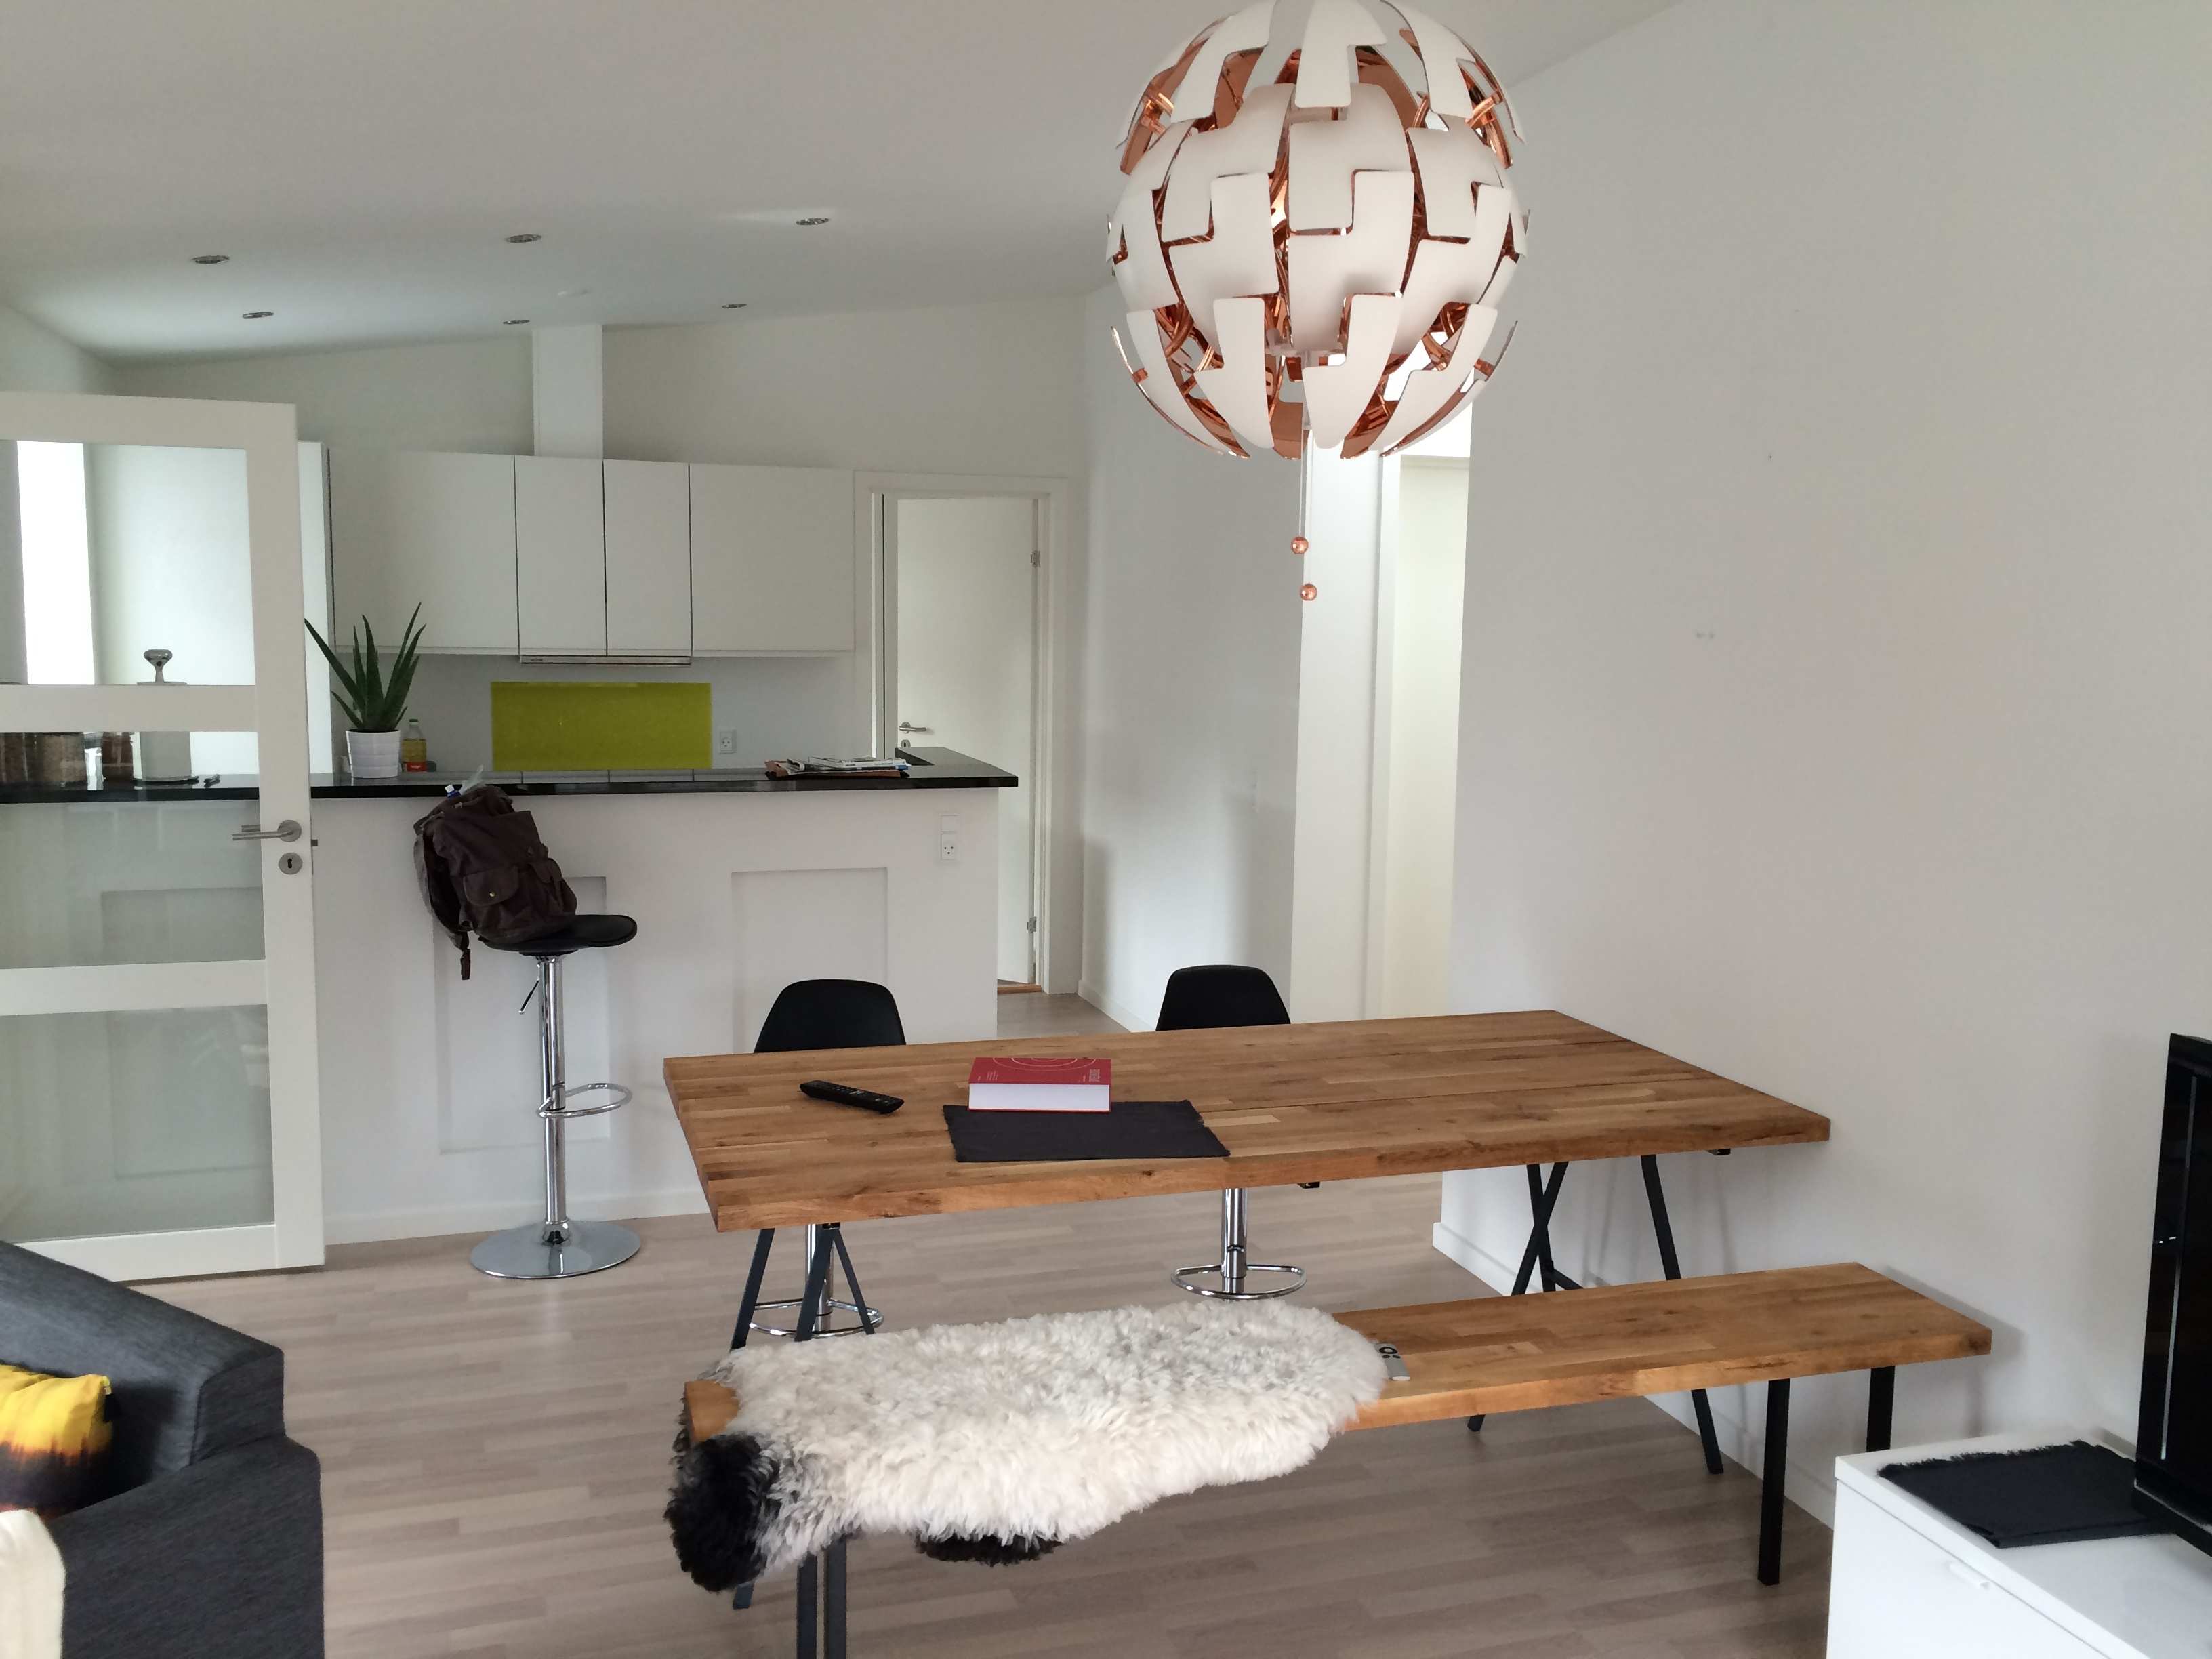
\includegraphics[width=.4\textwidth]{figures/roomOriginal.jpg}}
\end{figure}
\begin{figure}
\centering
\subfigure[Room1char]{\label{fig:Room1char}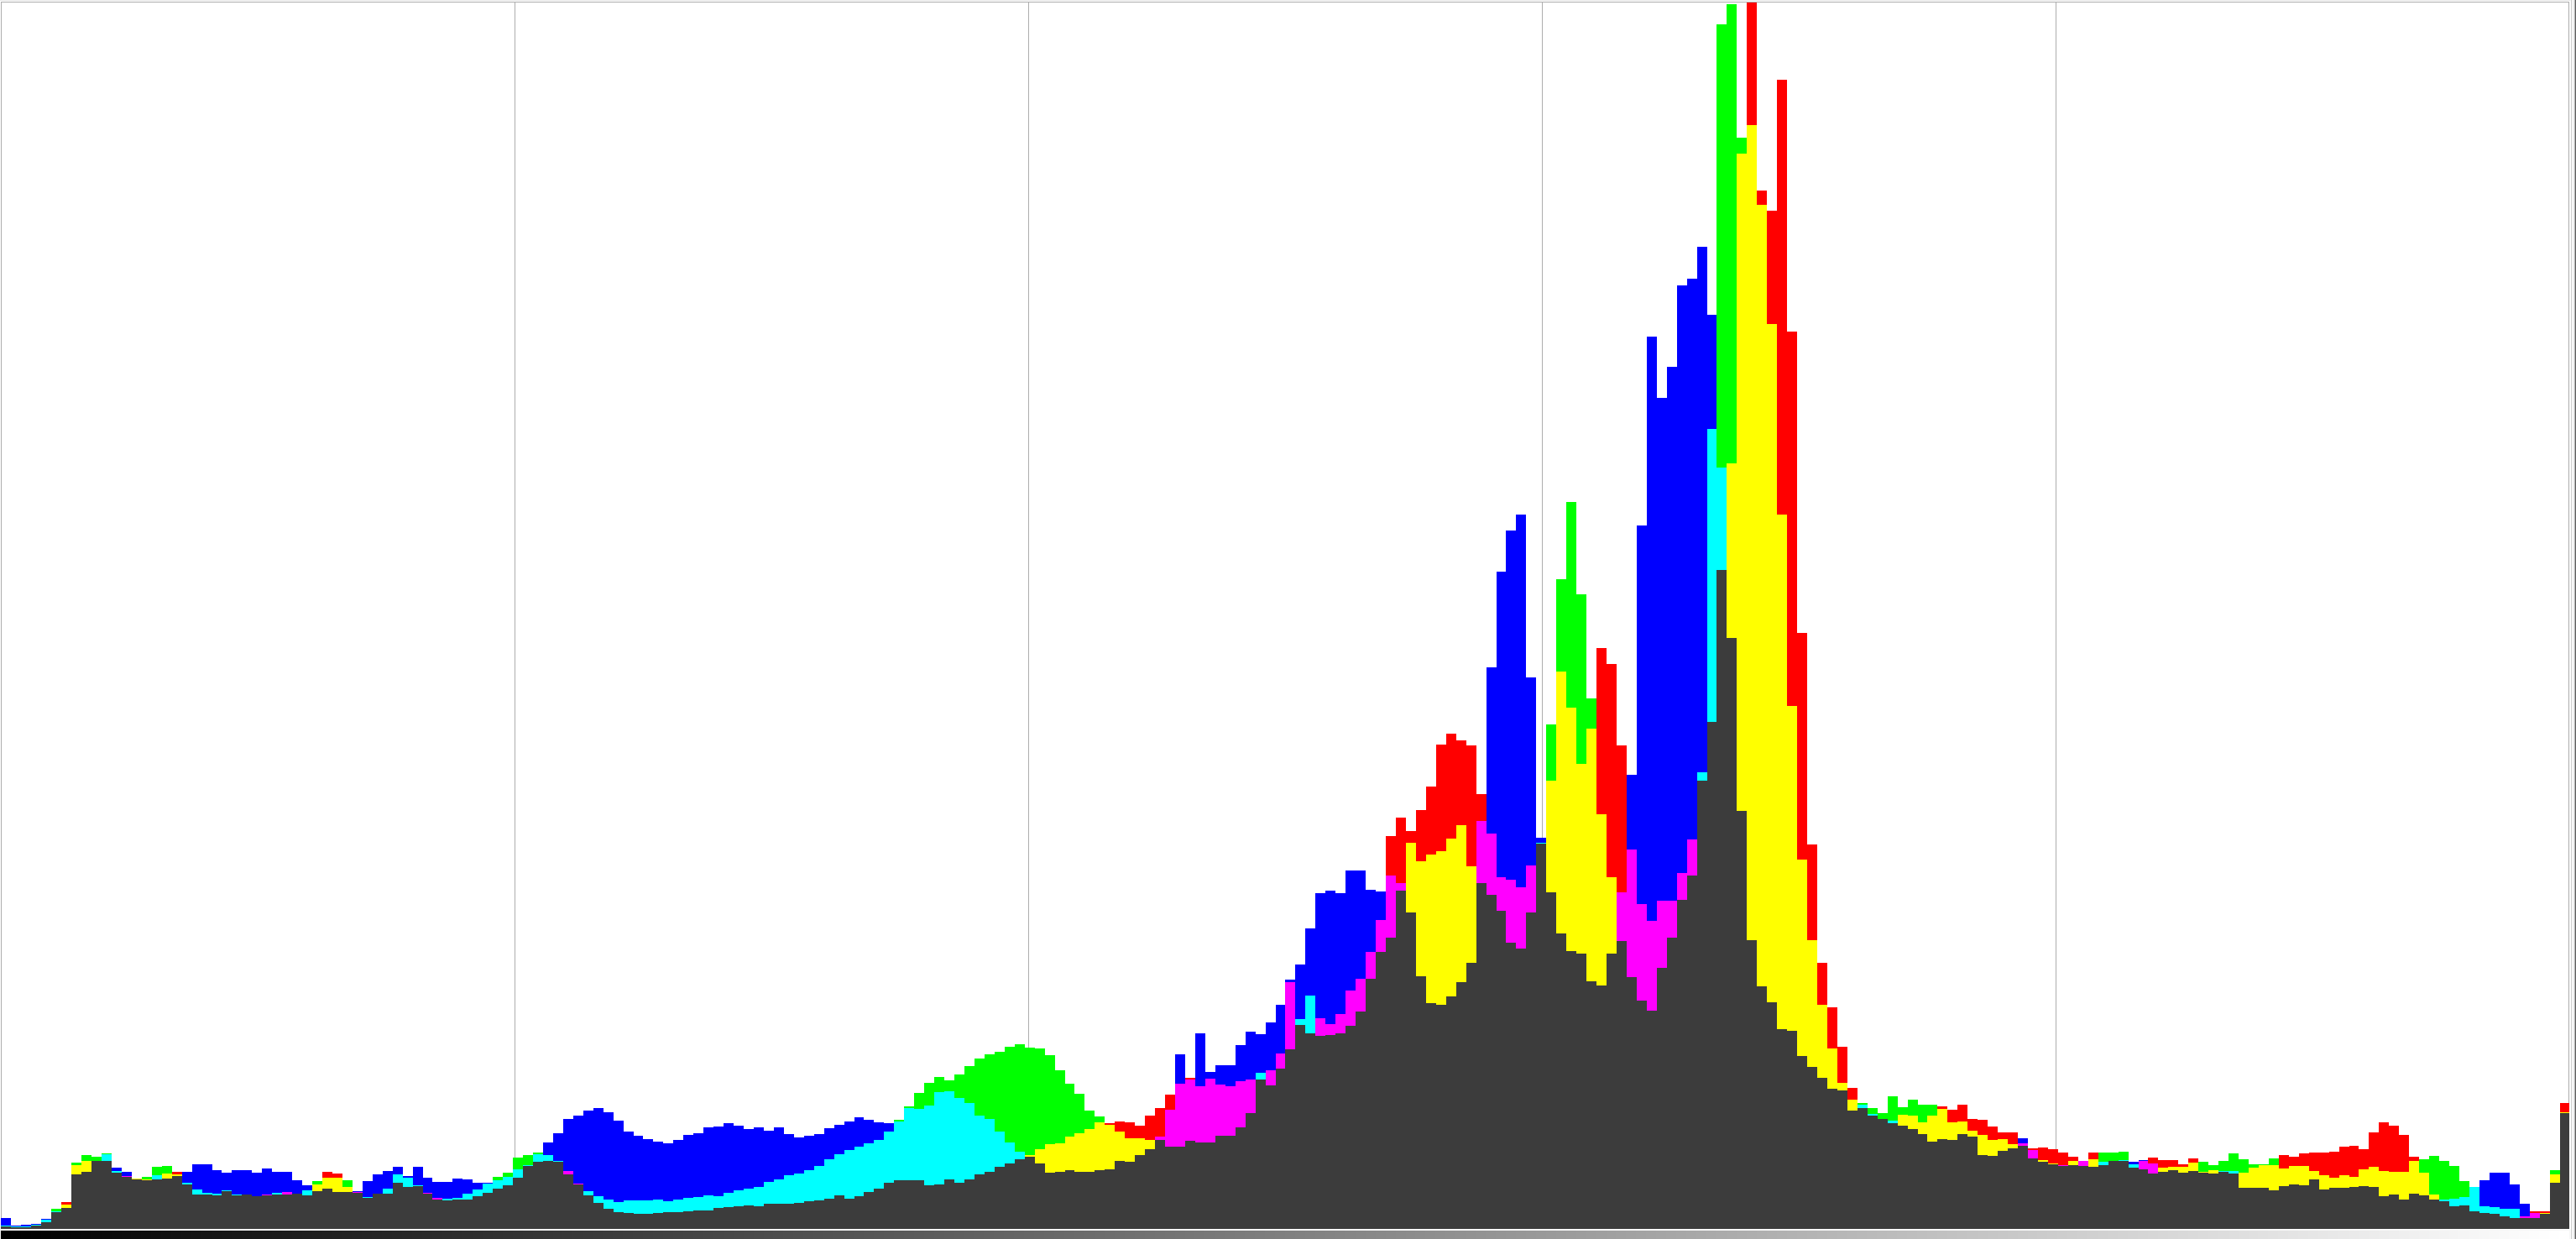
\includegraphics[width=.4\textwidth]{figures/room1char.png}}
\subfigure[RoomIntro]{\label{fig:RoomIntro}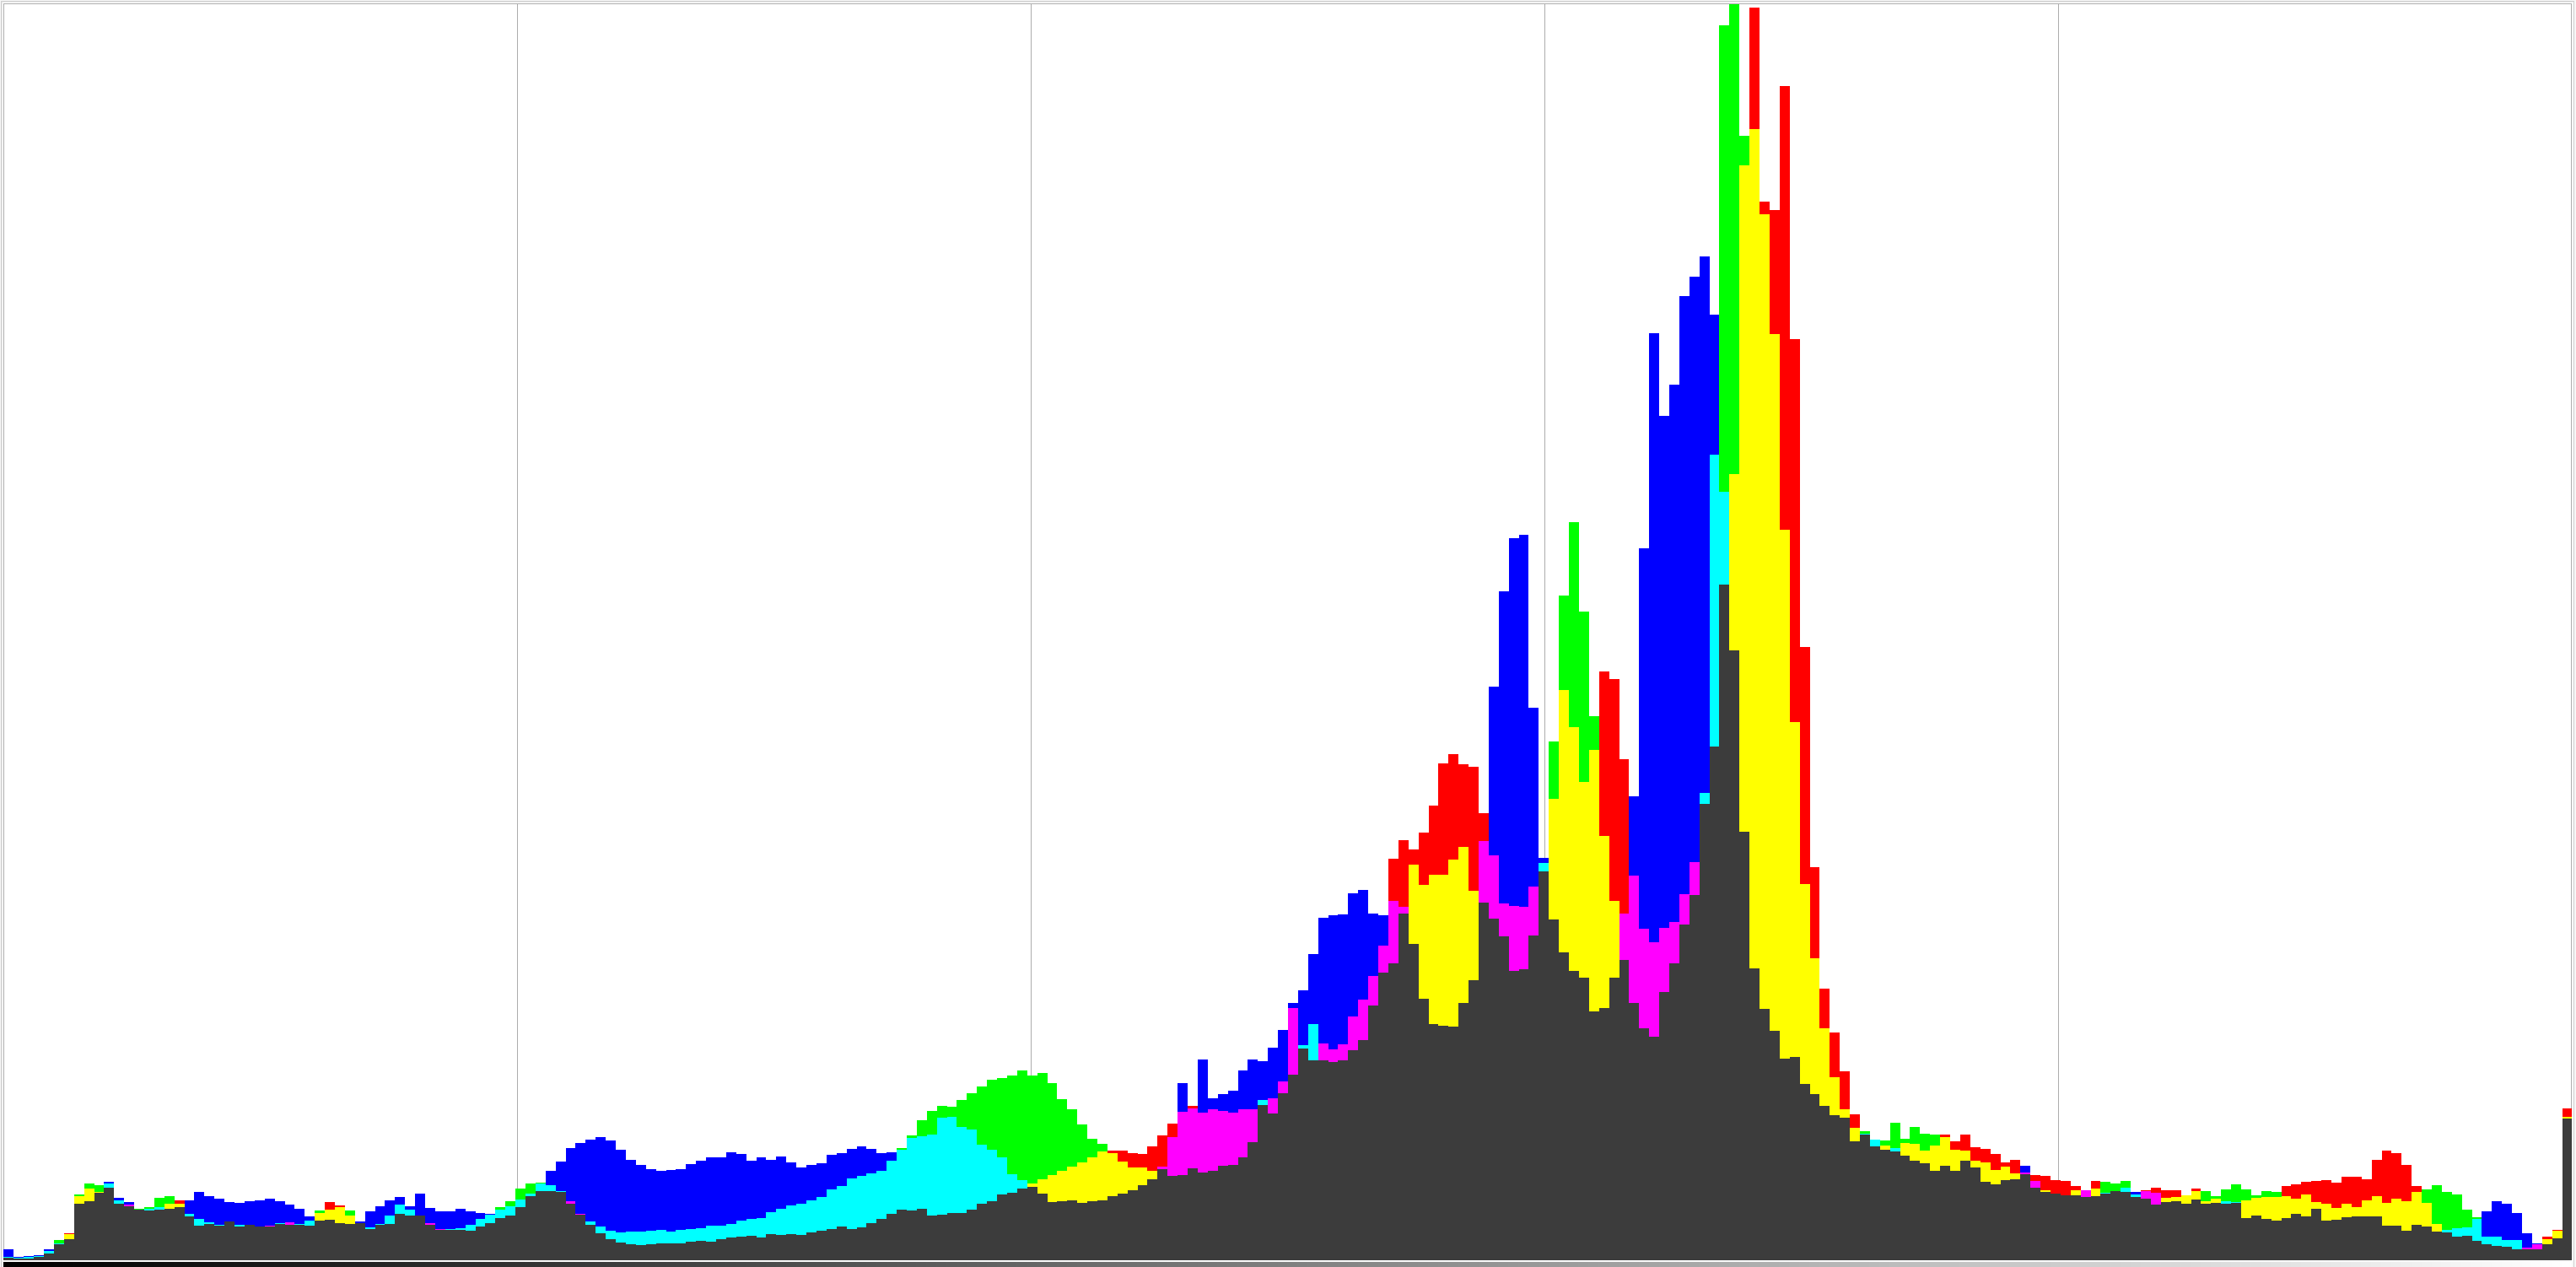
\includegraphics[width=.4\textwidth]{figures/roomEncodedIntroToSteg.png}}
\caption{Sammenligning af colour histogram}
\end{figure}
\end{frame}

\subsection{LSB enhancing}
\begin{frame}{LSB enhancing}
	LSB enhancing
	\begin{itemize}
		\item eliminate all 7 high-level bits
		\item all bytes are now 0 or 1
		\item 0 stays 0 while 1 becomes 256
	\end{itemize}
\end{frame}

\begin{frame}{Room LSB enhanced}
\begin{figure}
\centering
\subfigure[Room]{\label{fig:Room}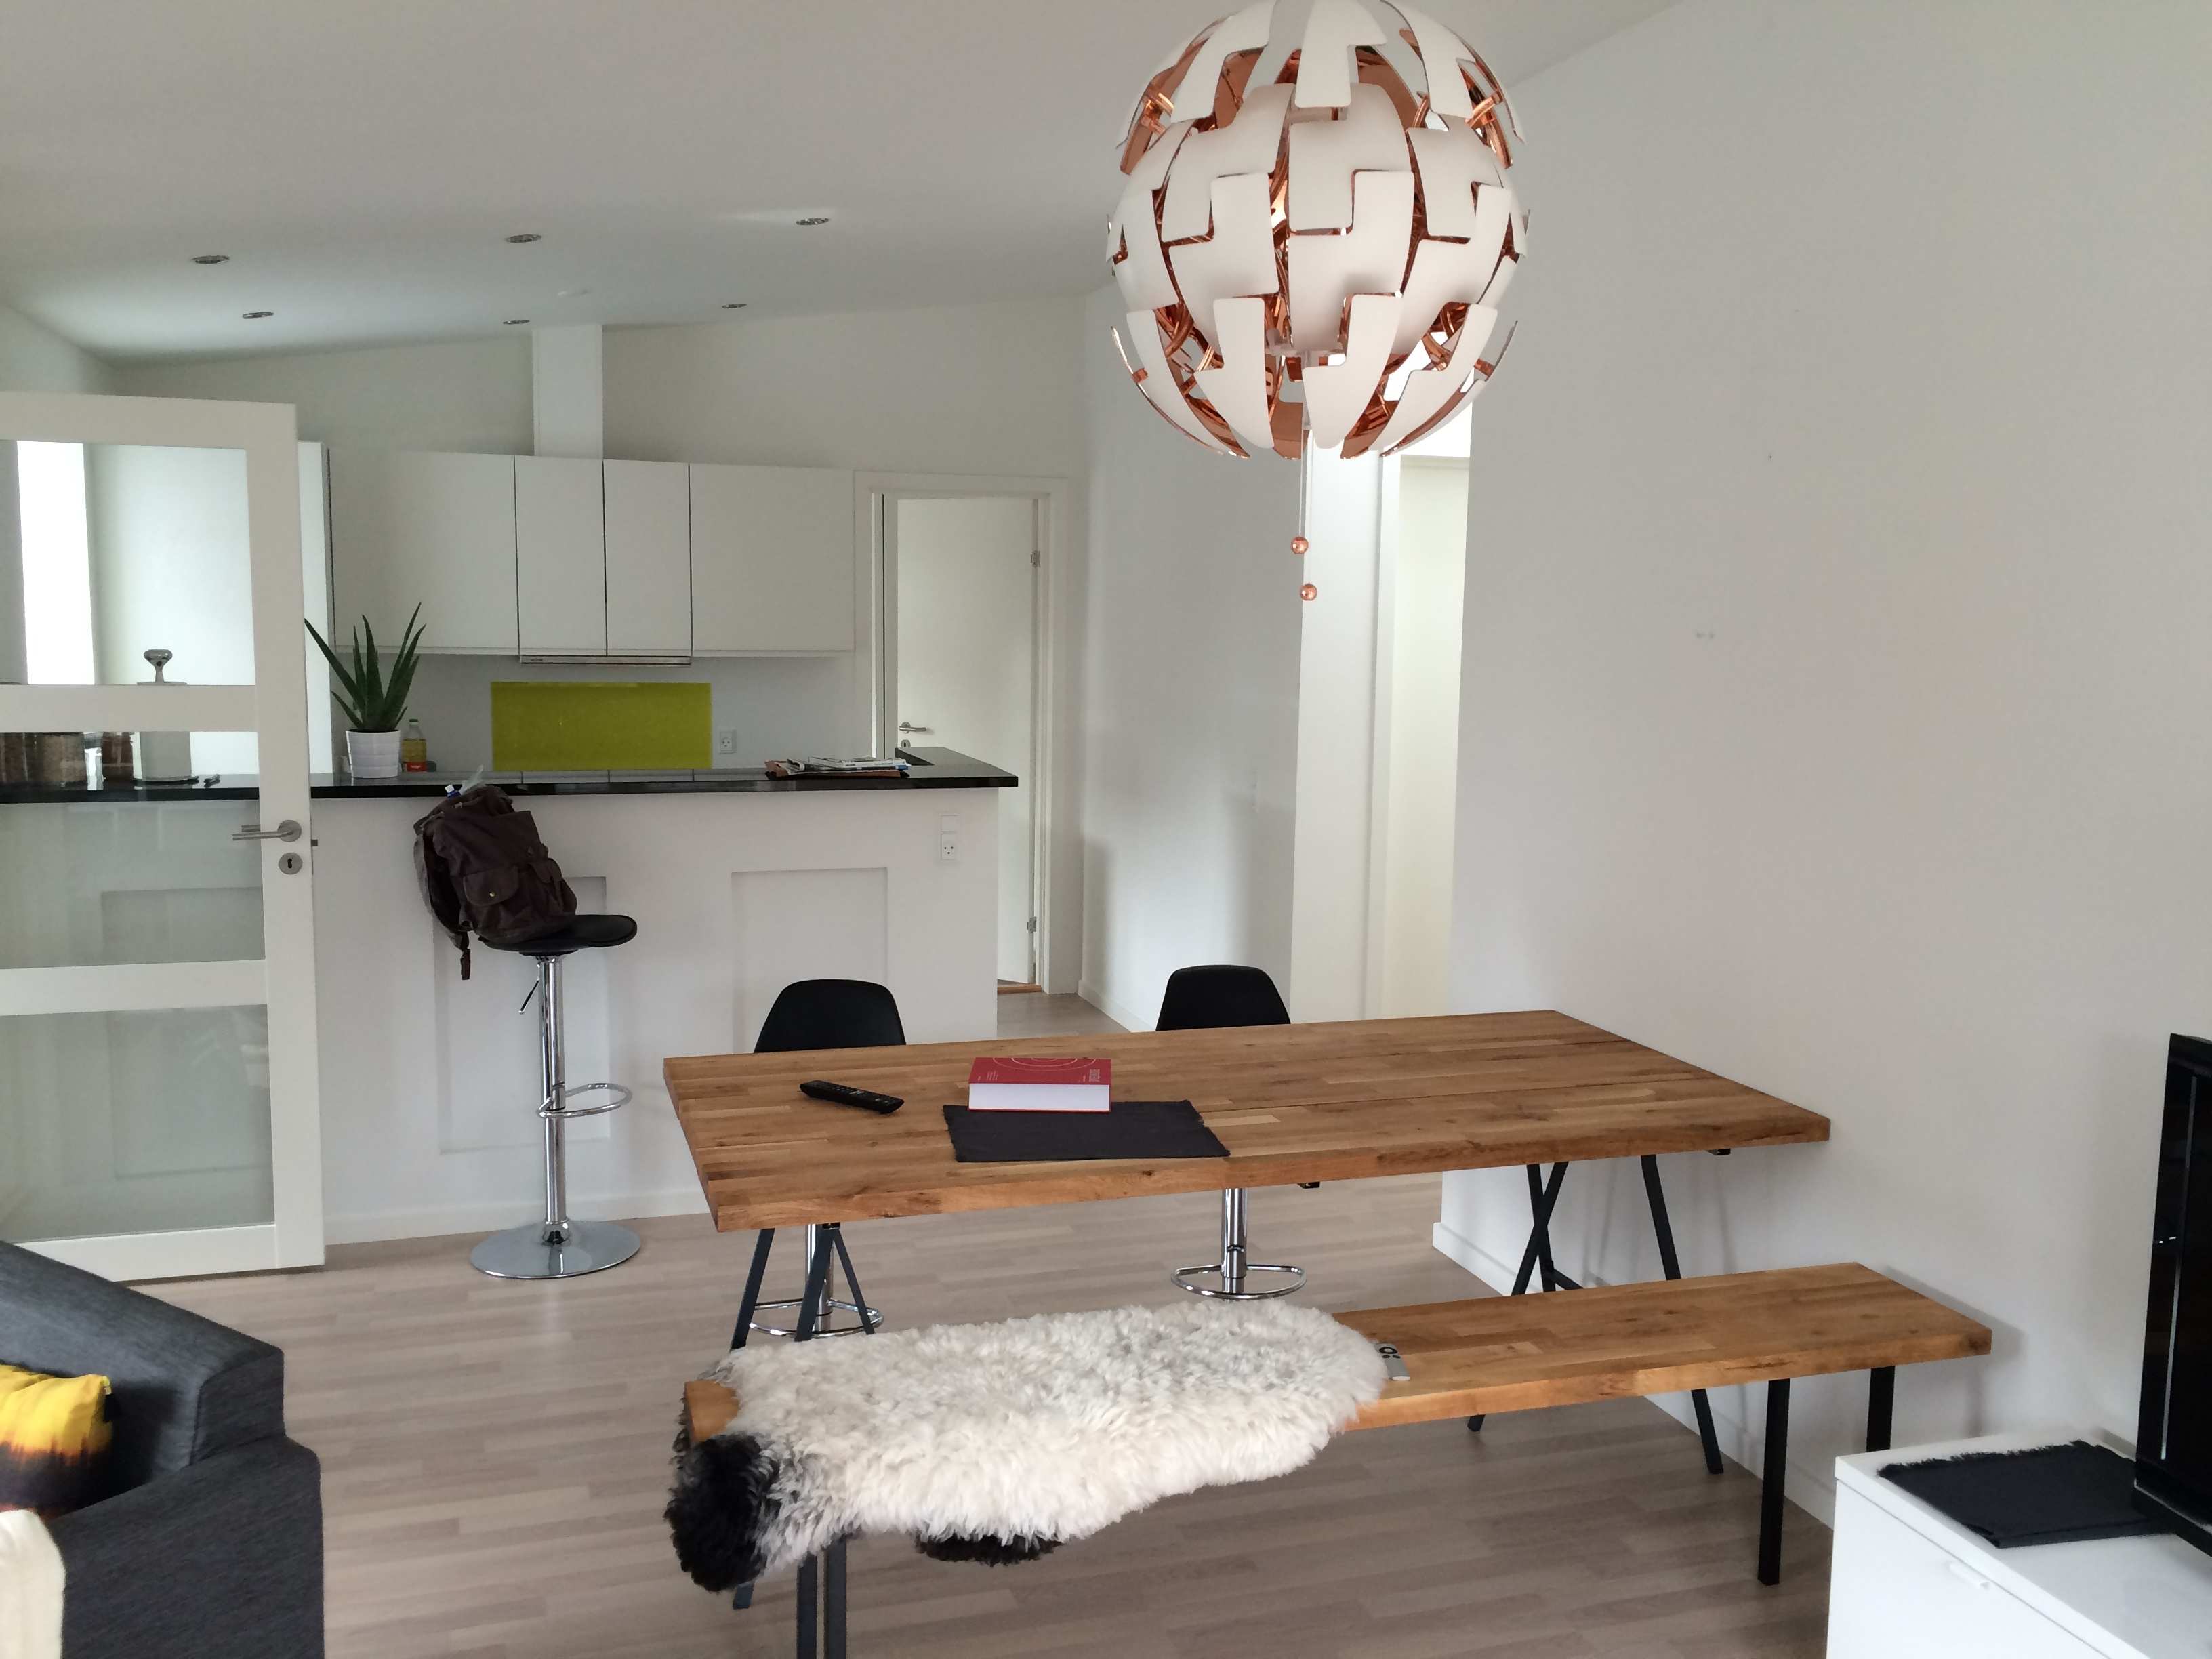
\includegraphics[width=.45\textwidth]{figures/roomOriginal.jpg}}
\subfigure[RoomLSB]{\label{fig:Room}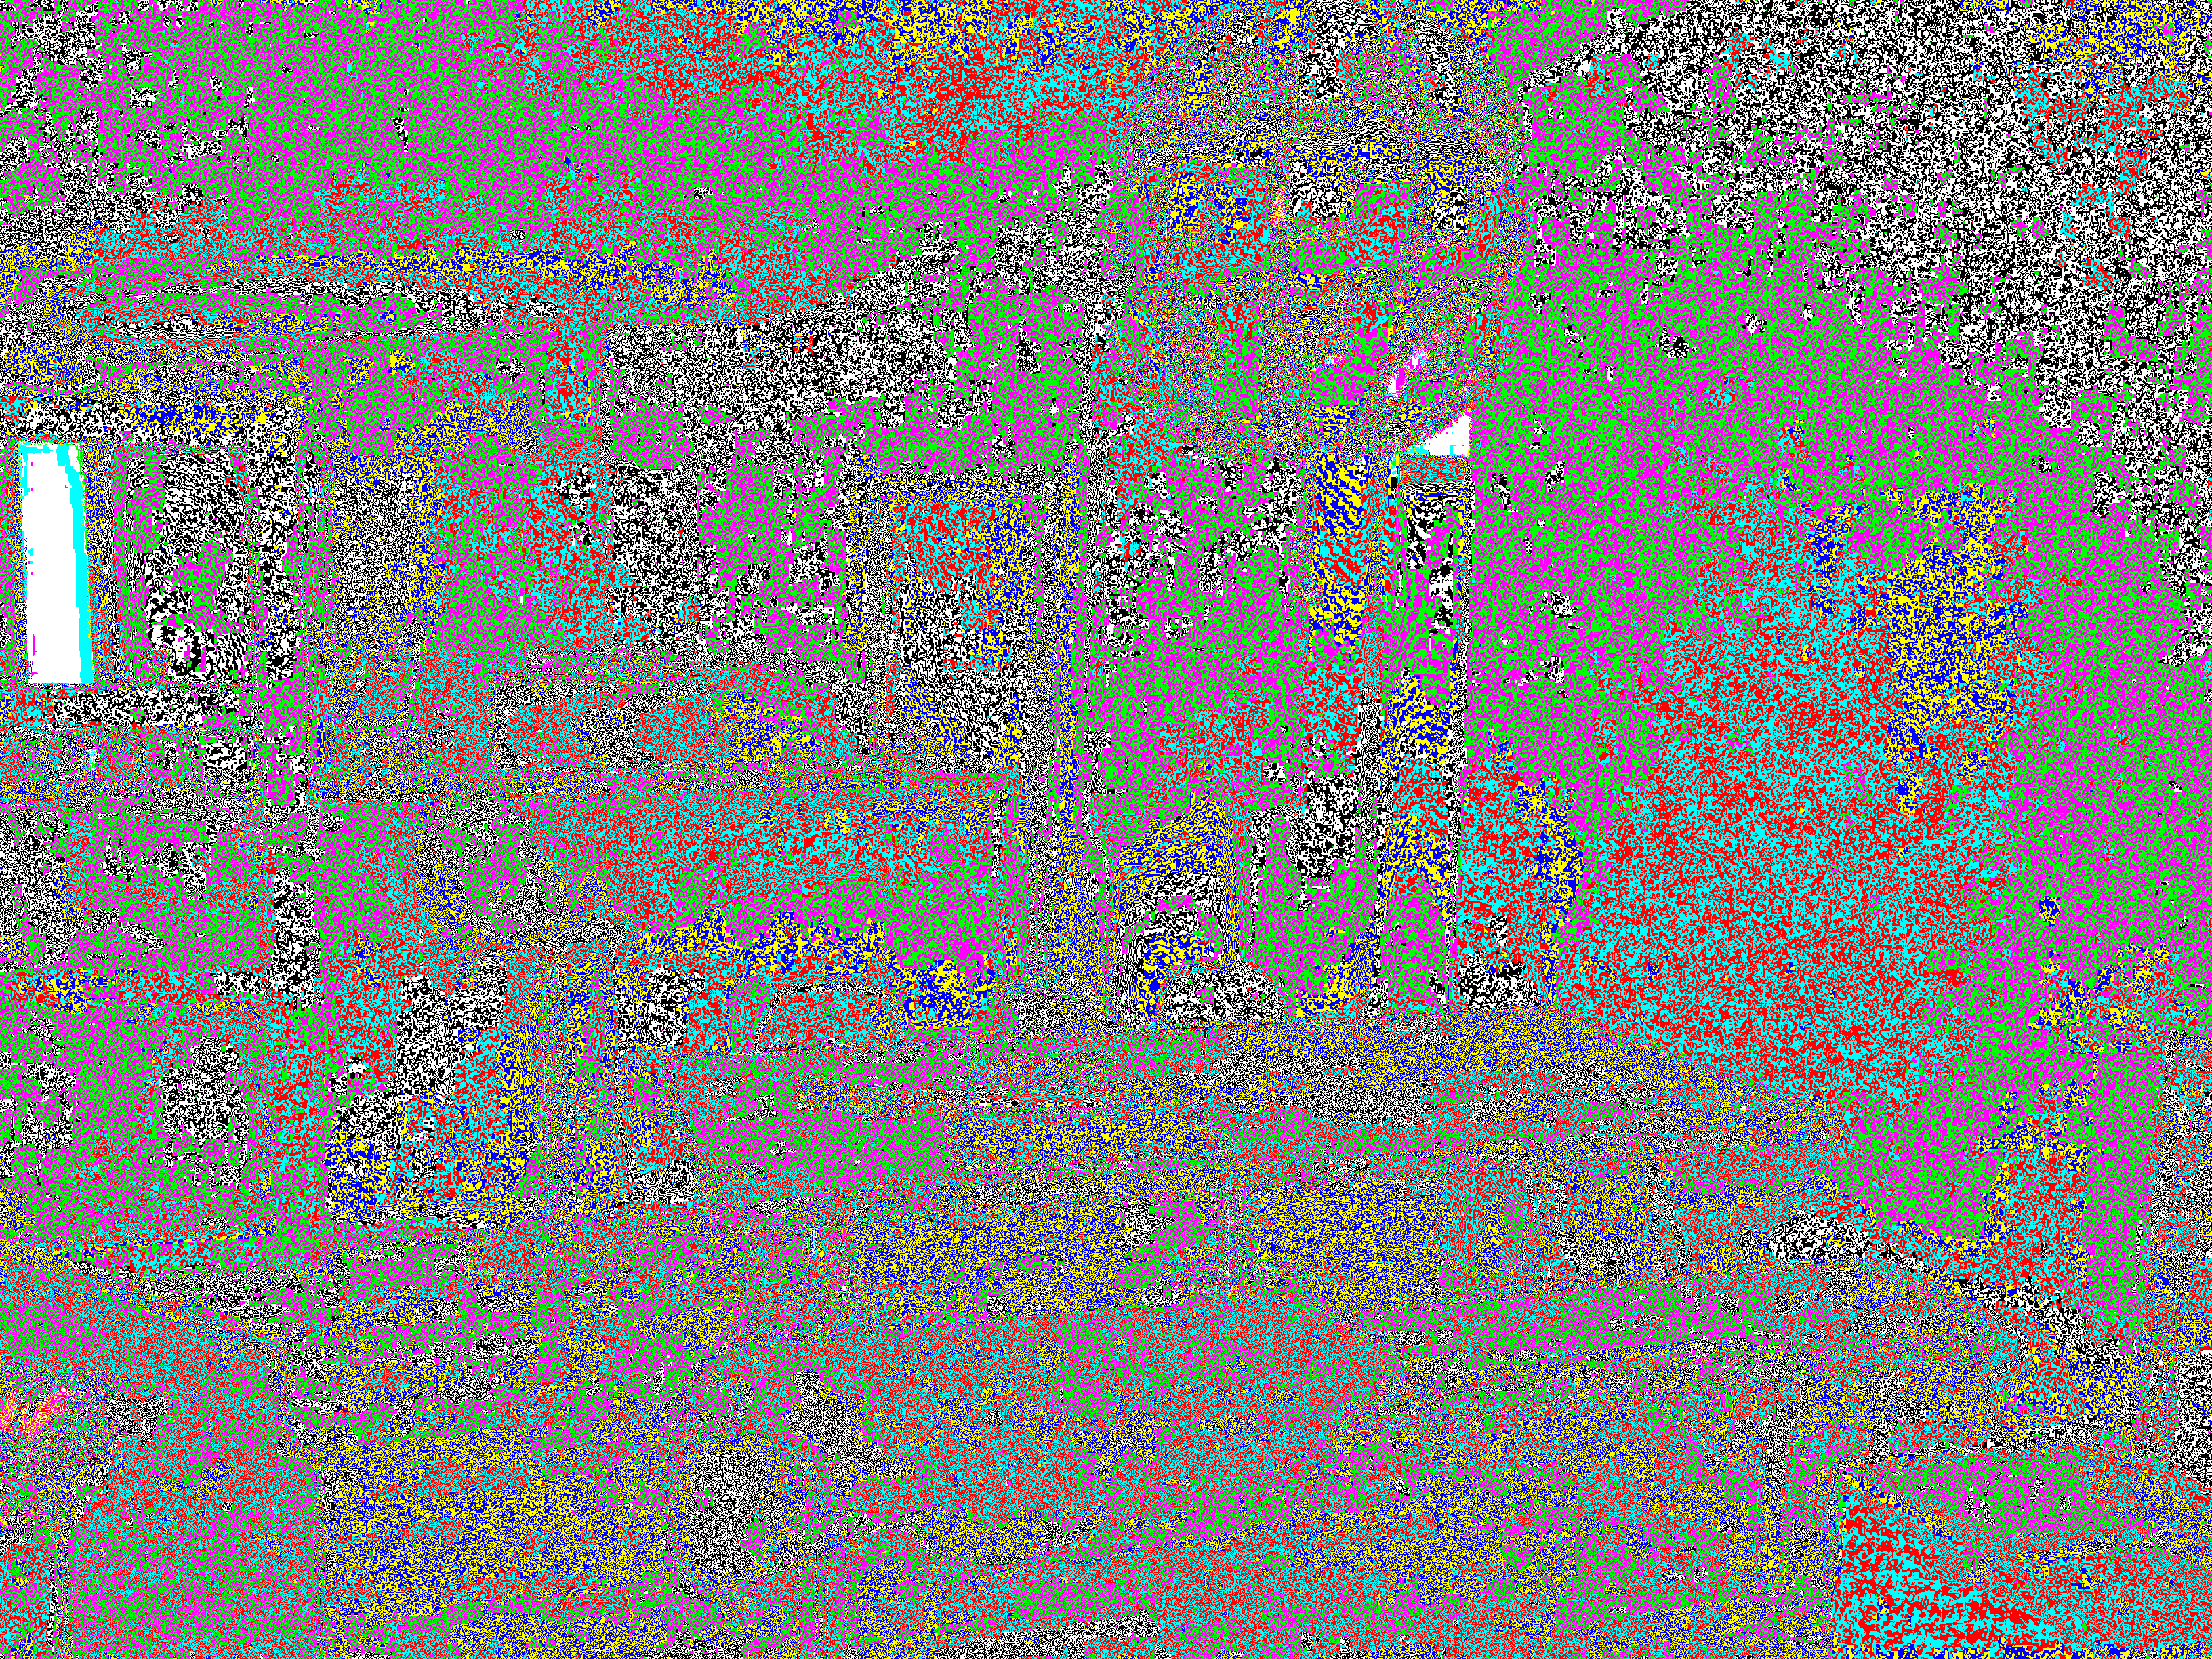
\includegraphics[width=.45\textwidth]{figures/roomOriLSB.png}}
\end{figure}
\end{frame}

\begin{frame}{Room LSB enhanced}
\begin{figure}
\centering
\subfigure[Room]{\label{fig:Room}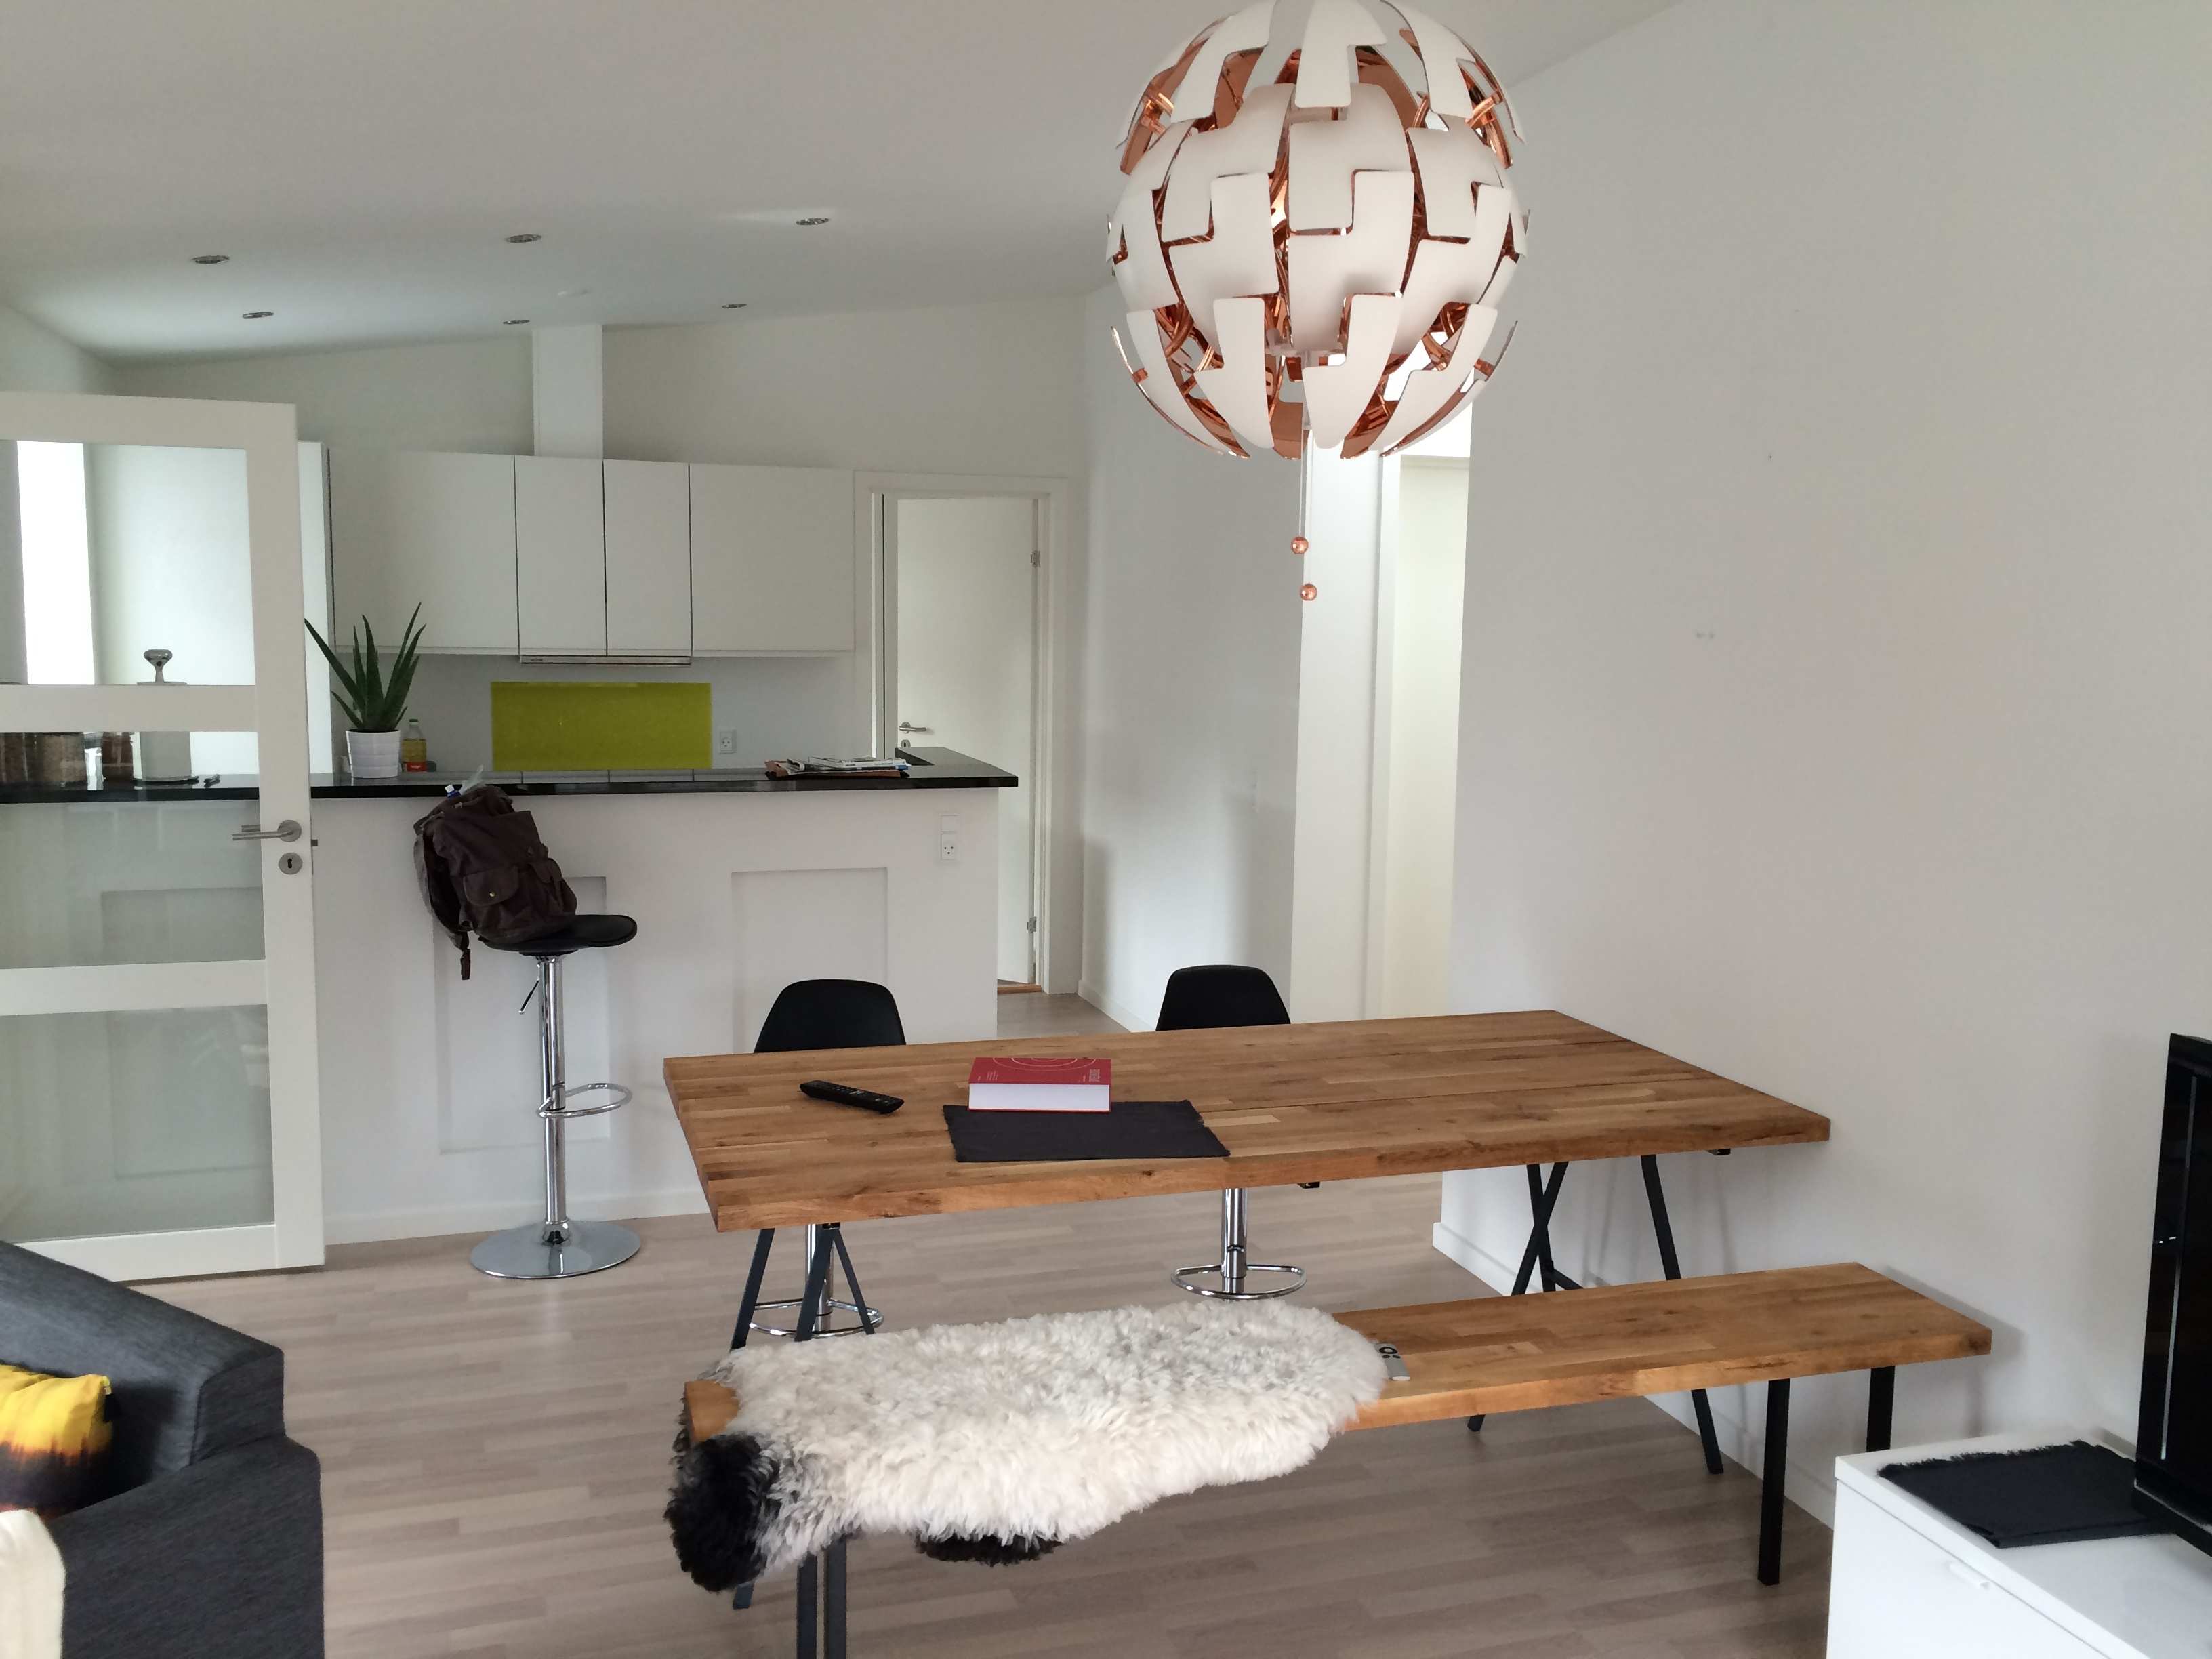
\includegraphics[width=.8\textwidth]{figures/roomOriginal.jpg}}
\end{figure}
\end{frame}

\begin{frame}{Room LSB enhanced}
\begin{figure}
\centering
\subfigure[RoomLSB]{\label{fig:Room}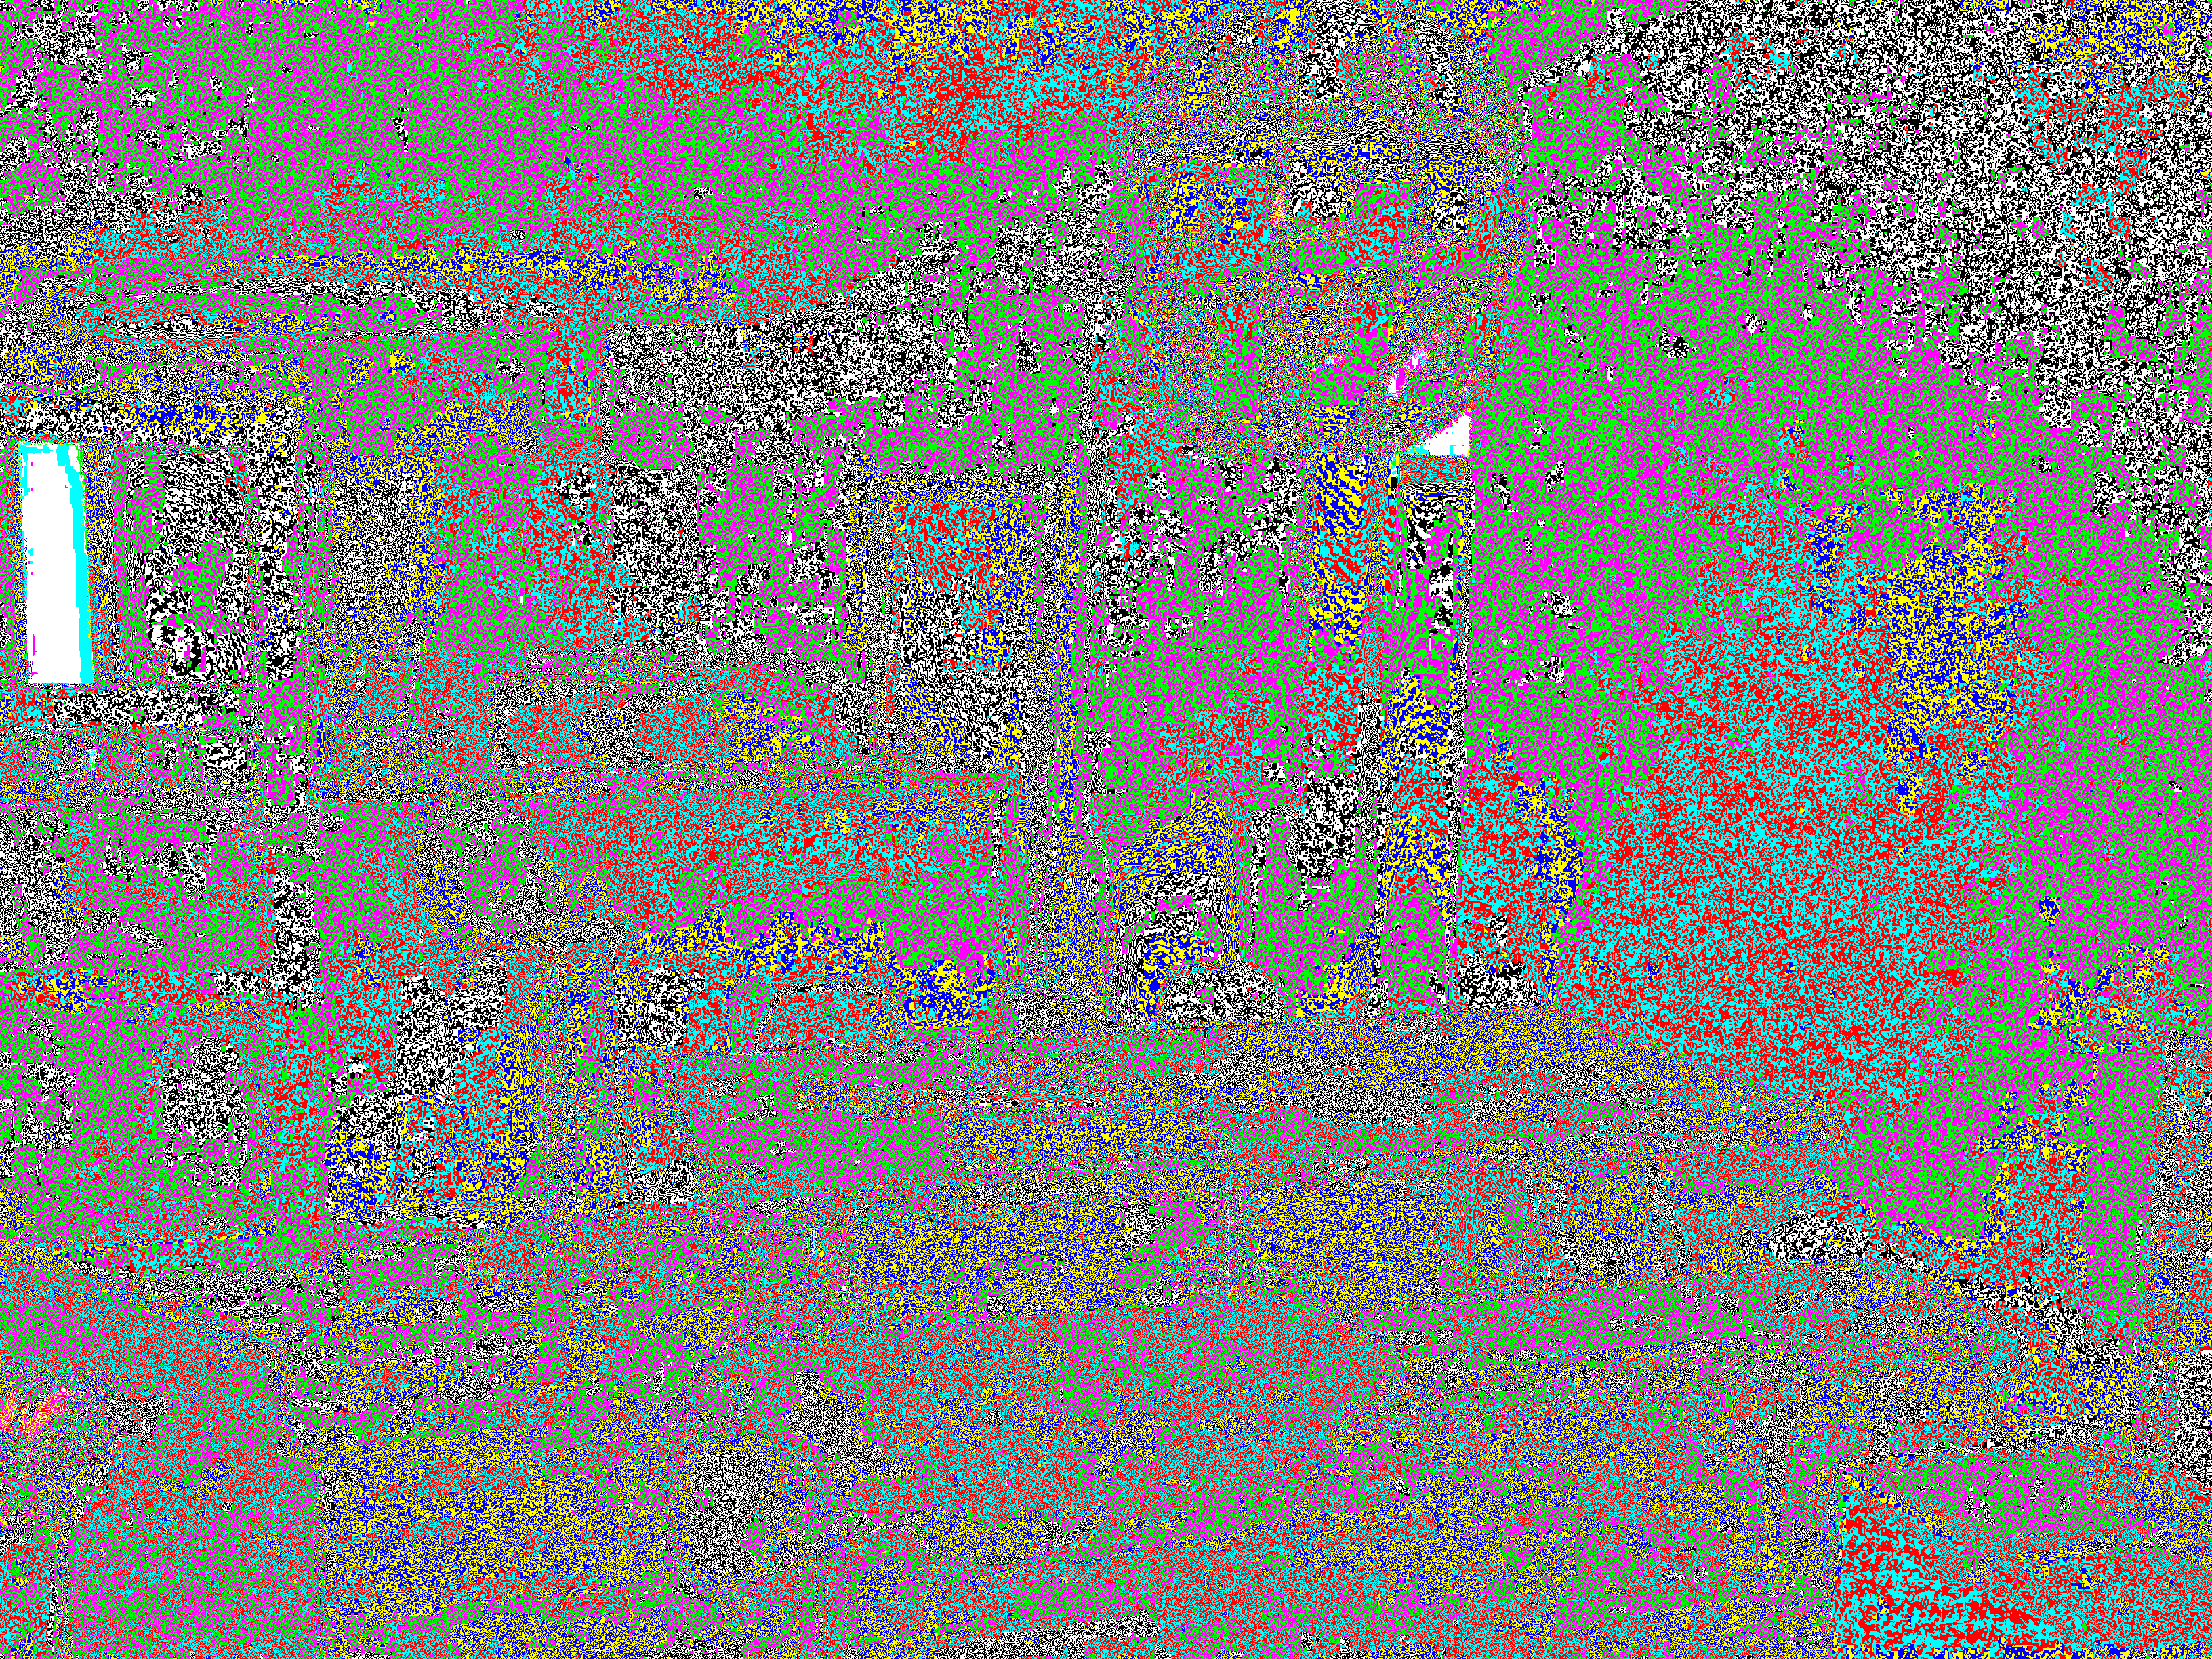
\includegraphics[width=.8\textwidth]{figures/roomOriLSB.png}}
\end{figure}
\end{frame}

\begin{frame}{Room encoded LSB enhanced}
\begin{figure}
\centering
\subfigure[RoomLSB]{\label{fig:Room}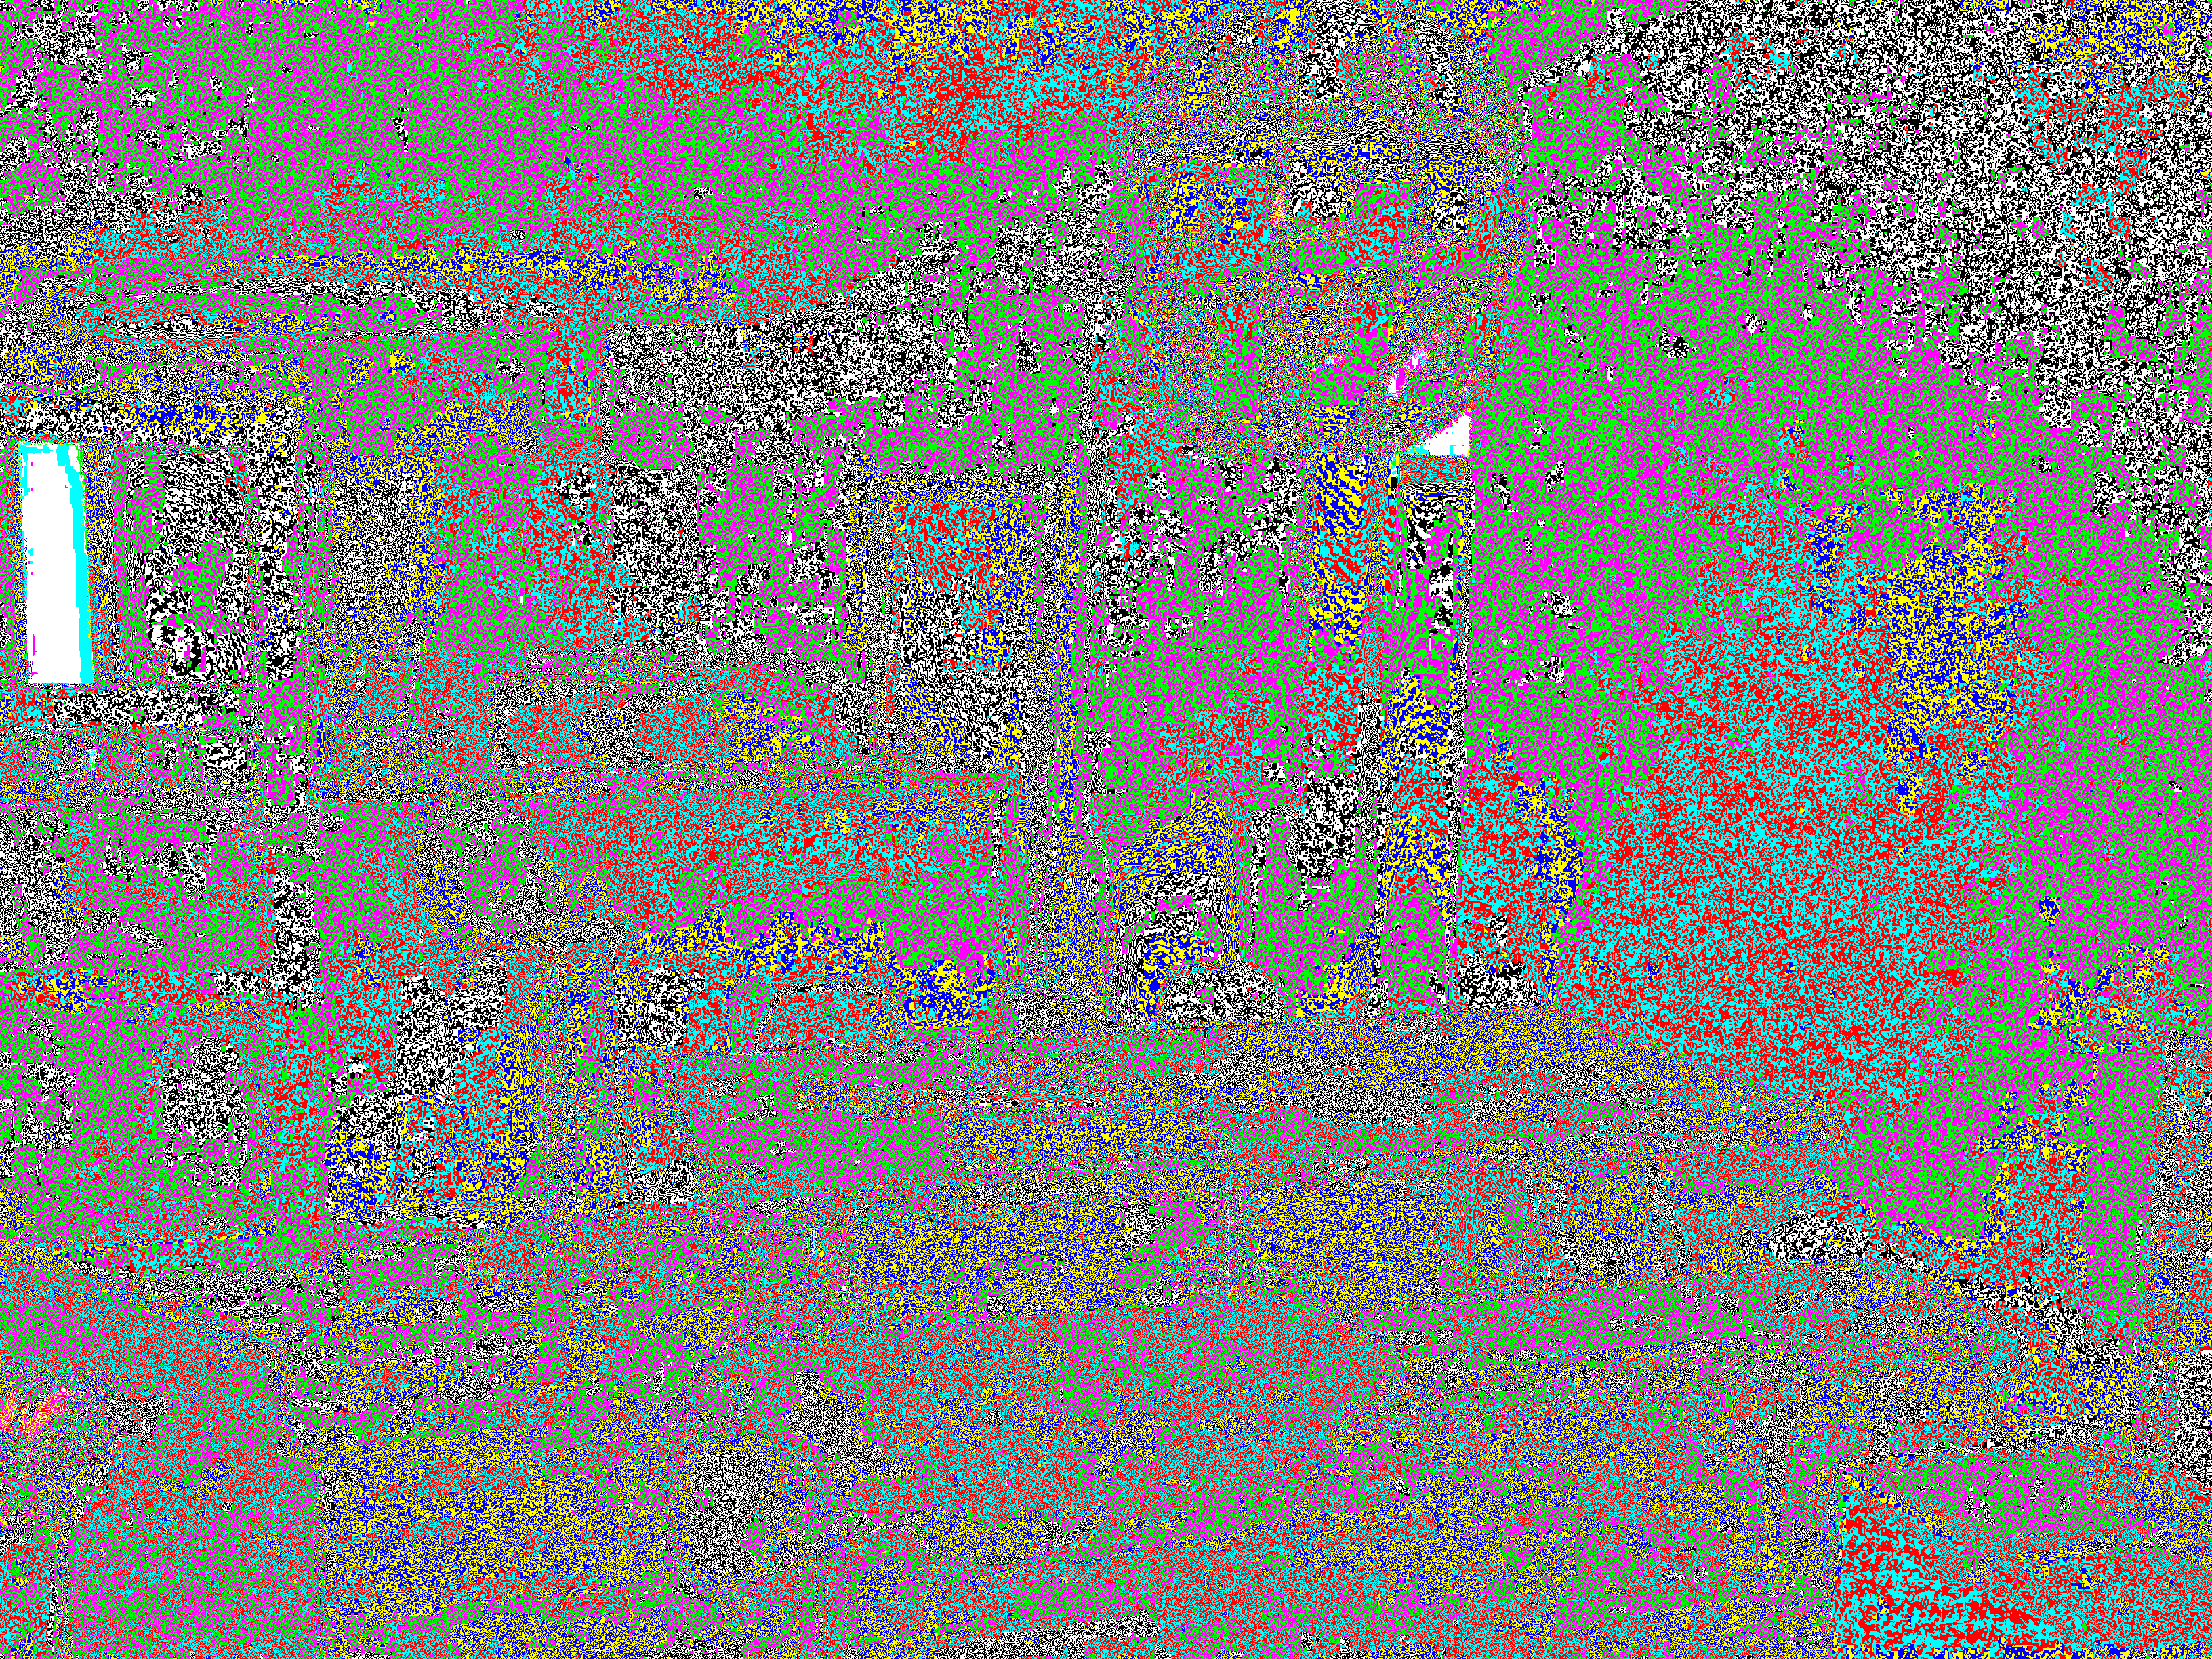
\includegraphics[width=.45\textwidth]{figures/roomOriLSB.png}}
\subfigure[RoomIntroLSB]{\label{fig:Room}
\includegraphics[width=.45\textwidth]{figures/roomIntroLSB.png}}
\end{figure}
\end{frame}

\subsection{Comparing image with original image}
\begin{frame}{looking at how images differ from original}
\begin{figure}
\centering
\subfigure[Room]{\label{fig:a}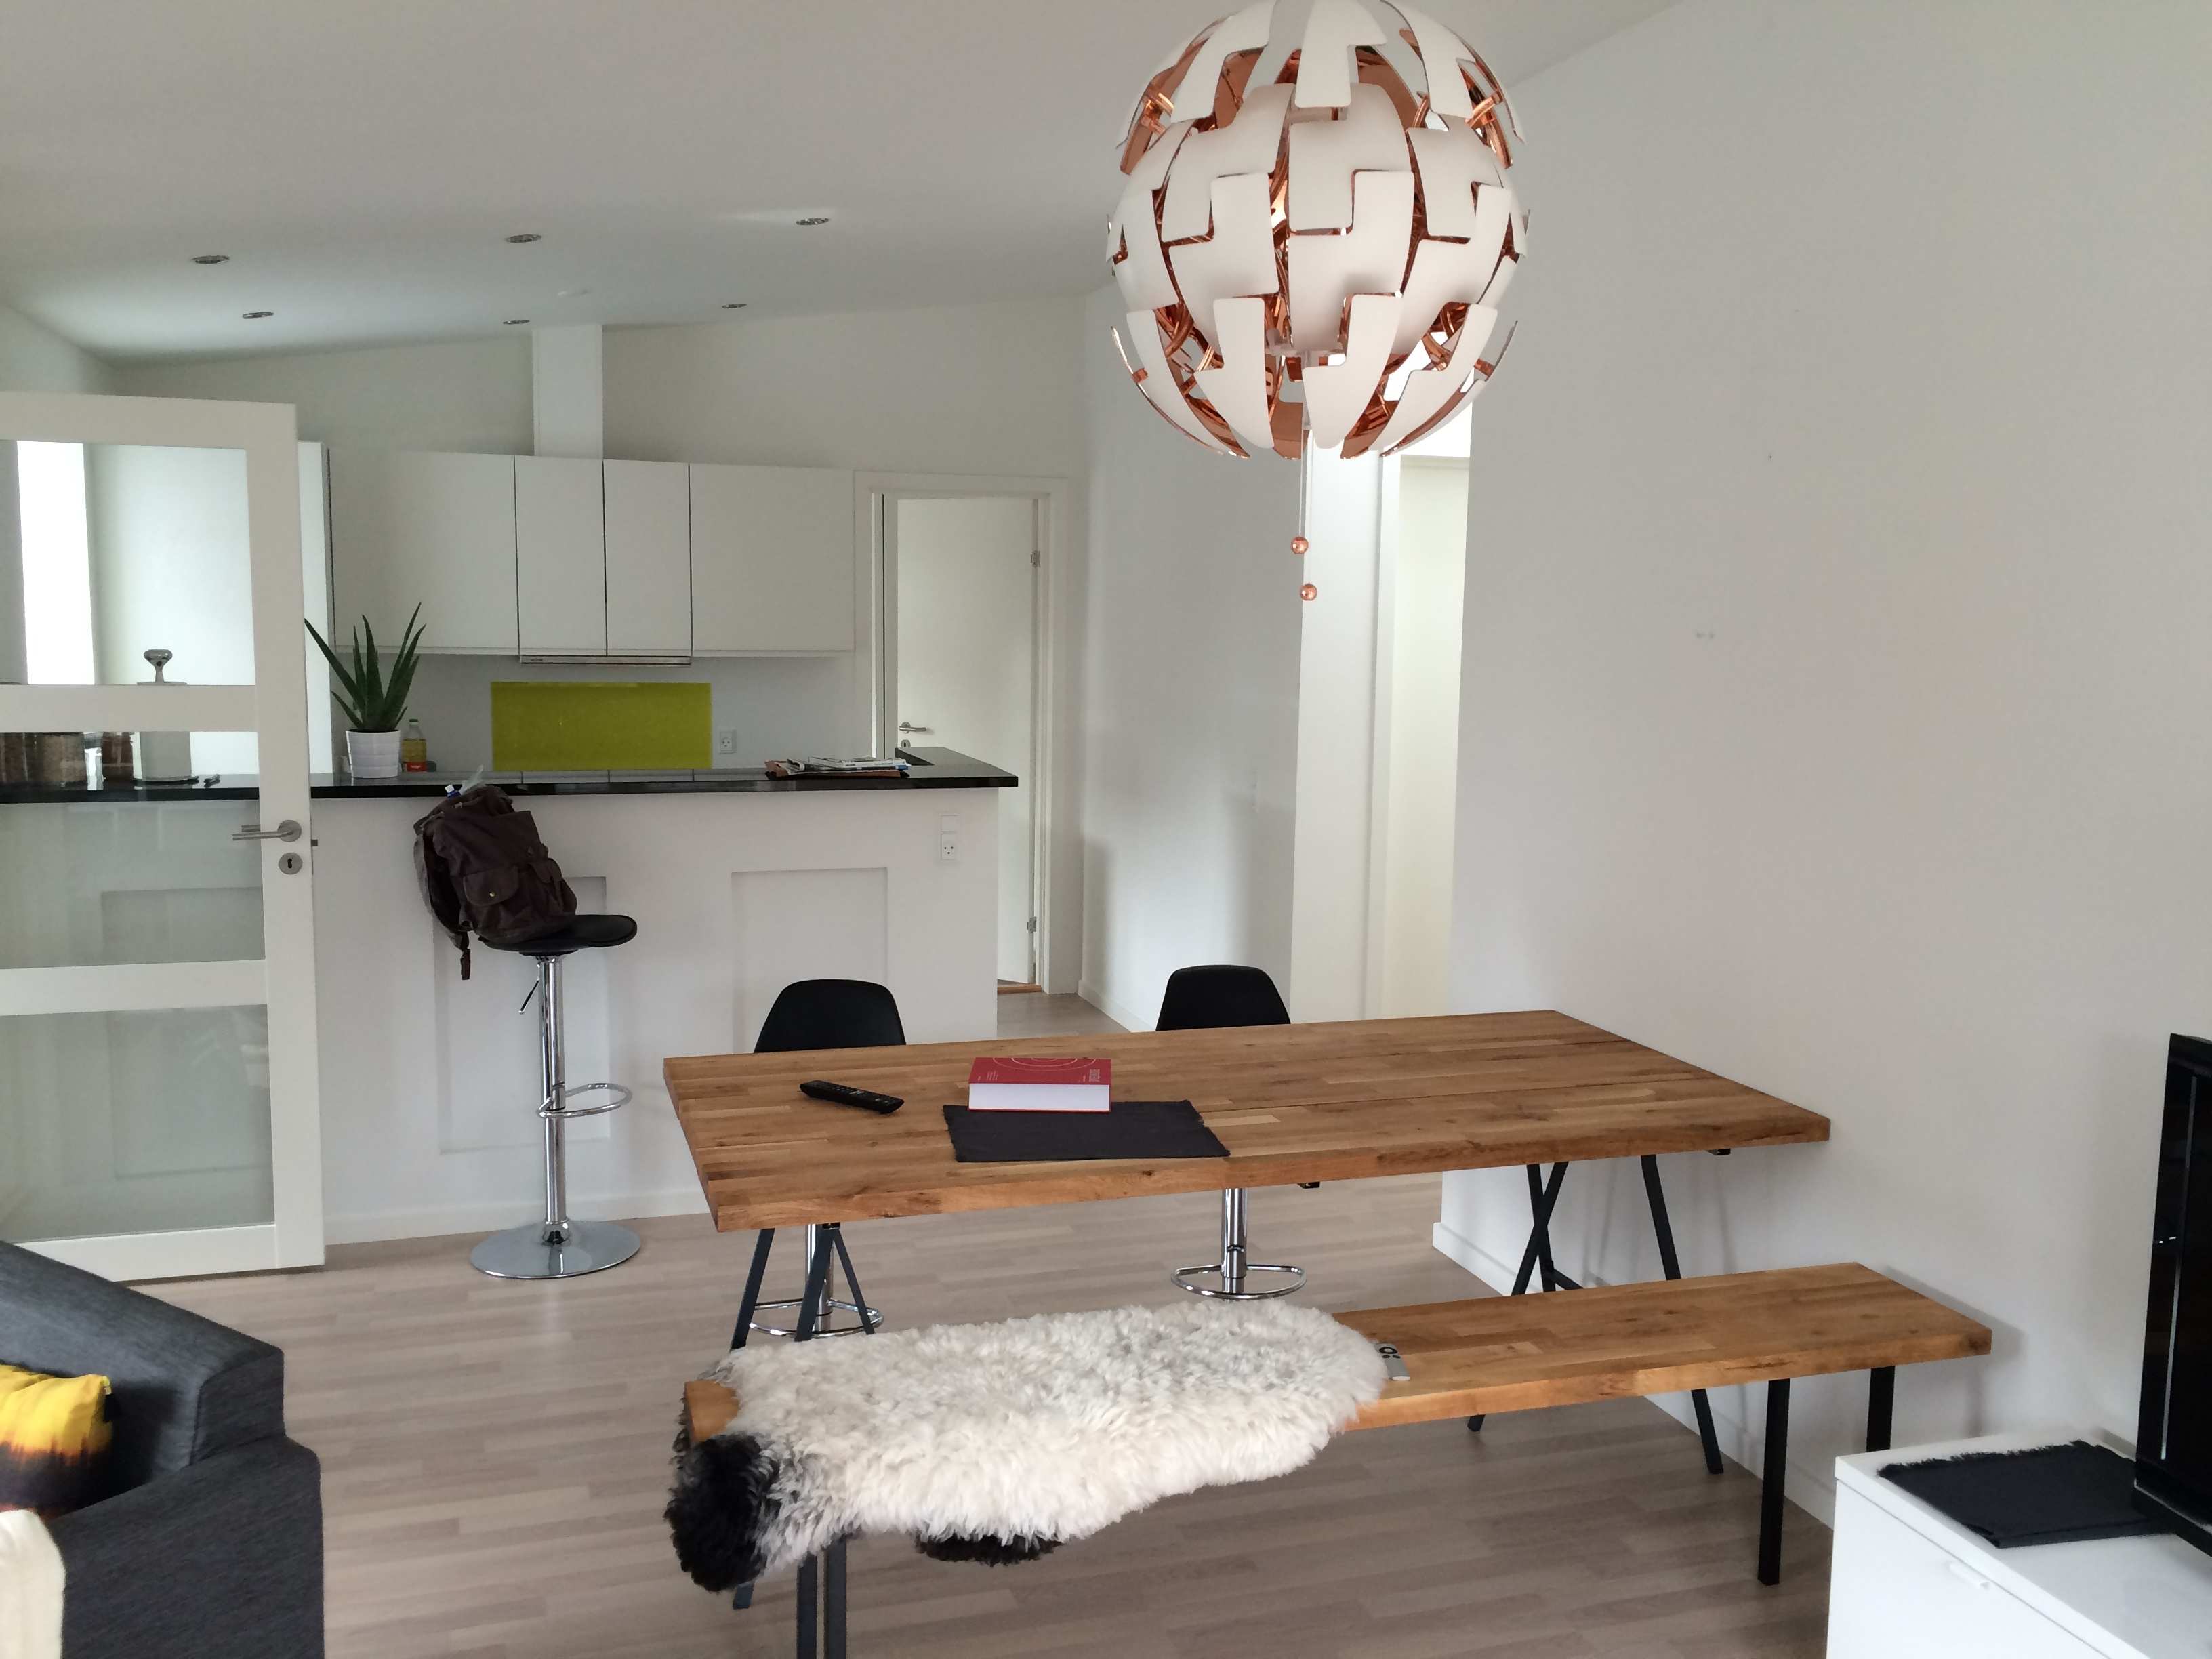
\includegraphics[width=.4\textwidth]{figures/roomOriginal.jpg}}
\subfigure[Room1char]{\label{fig:b}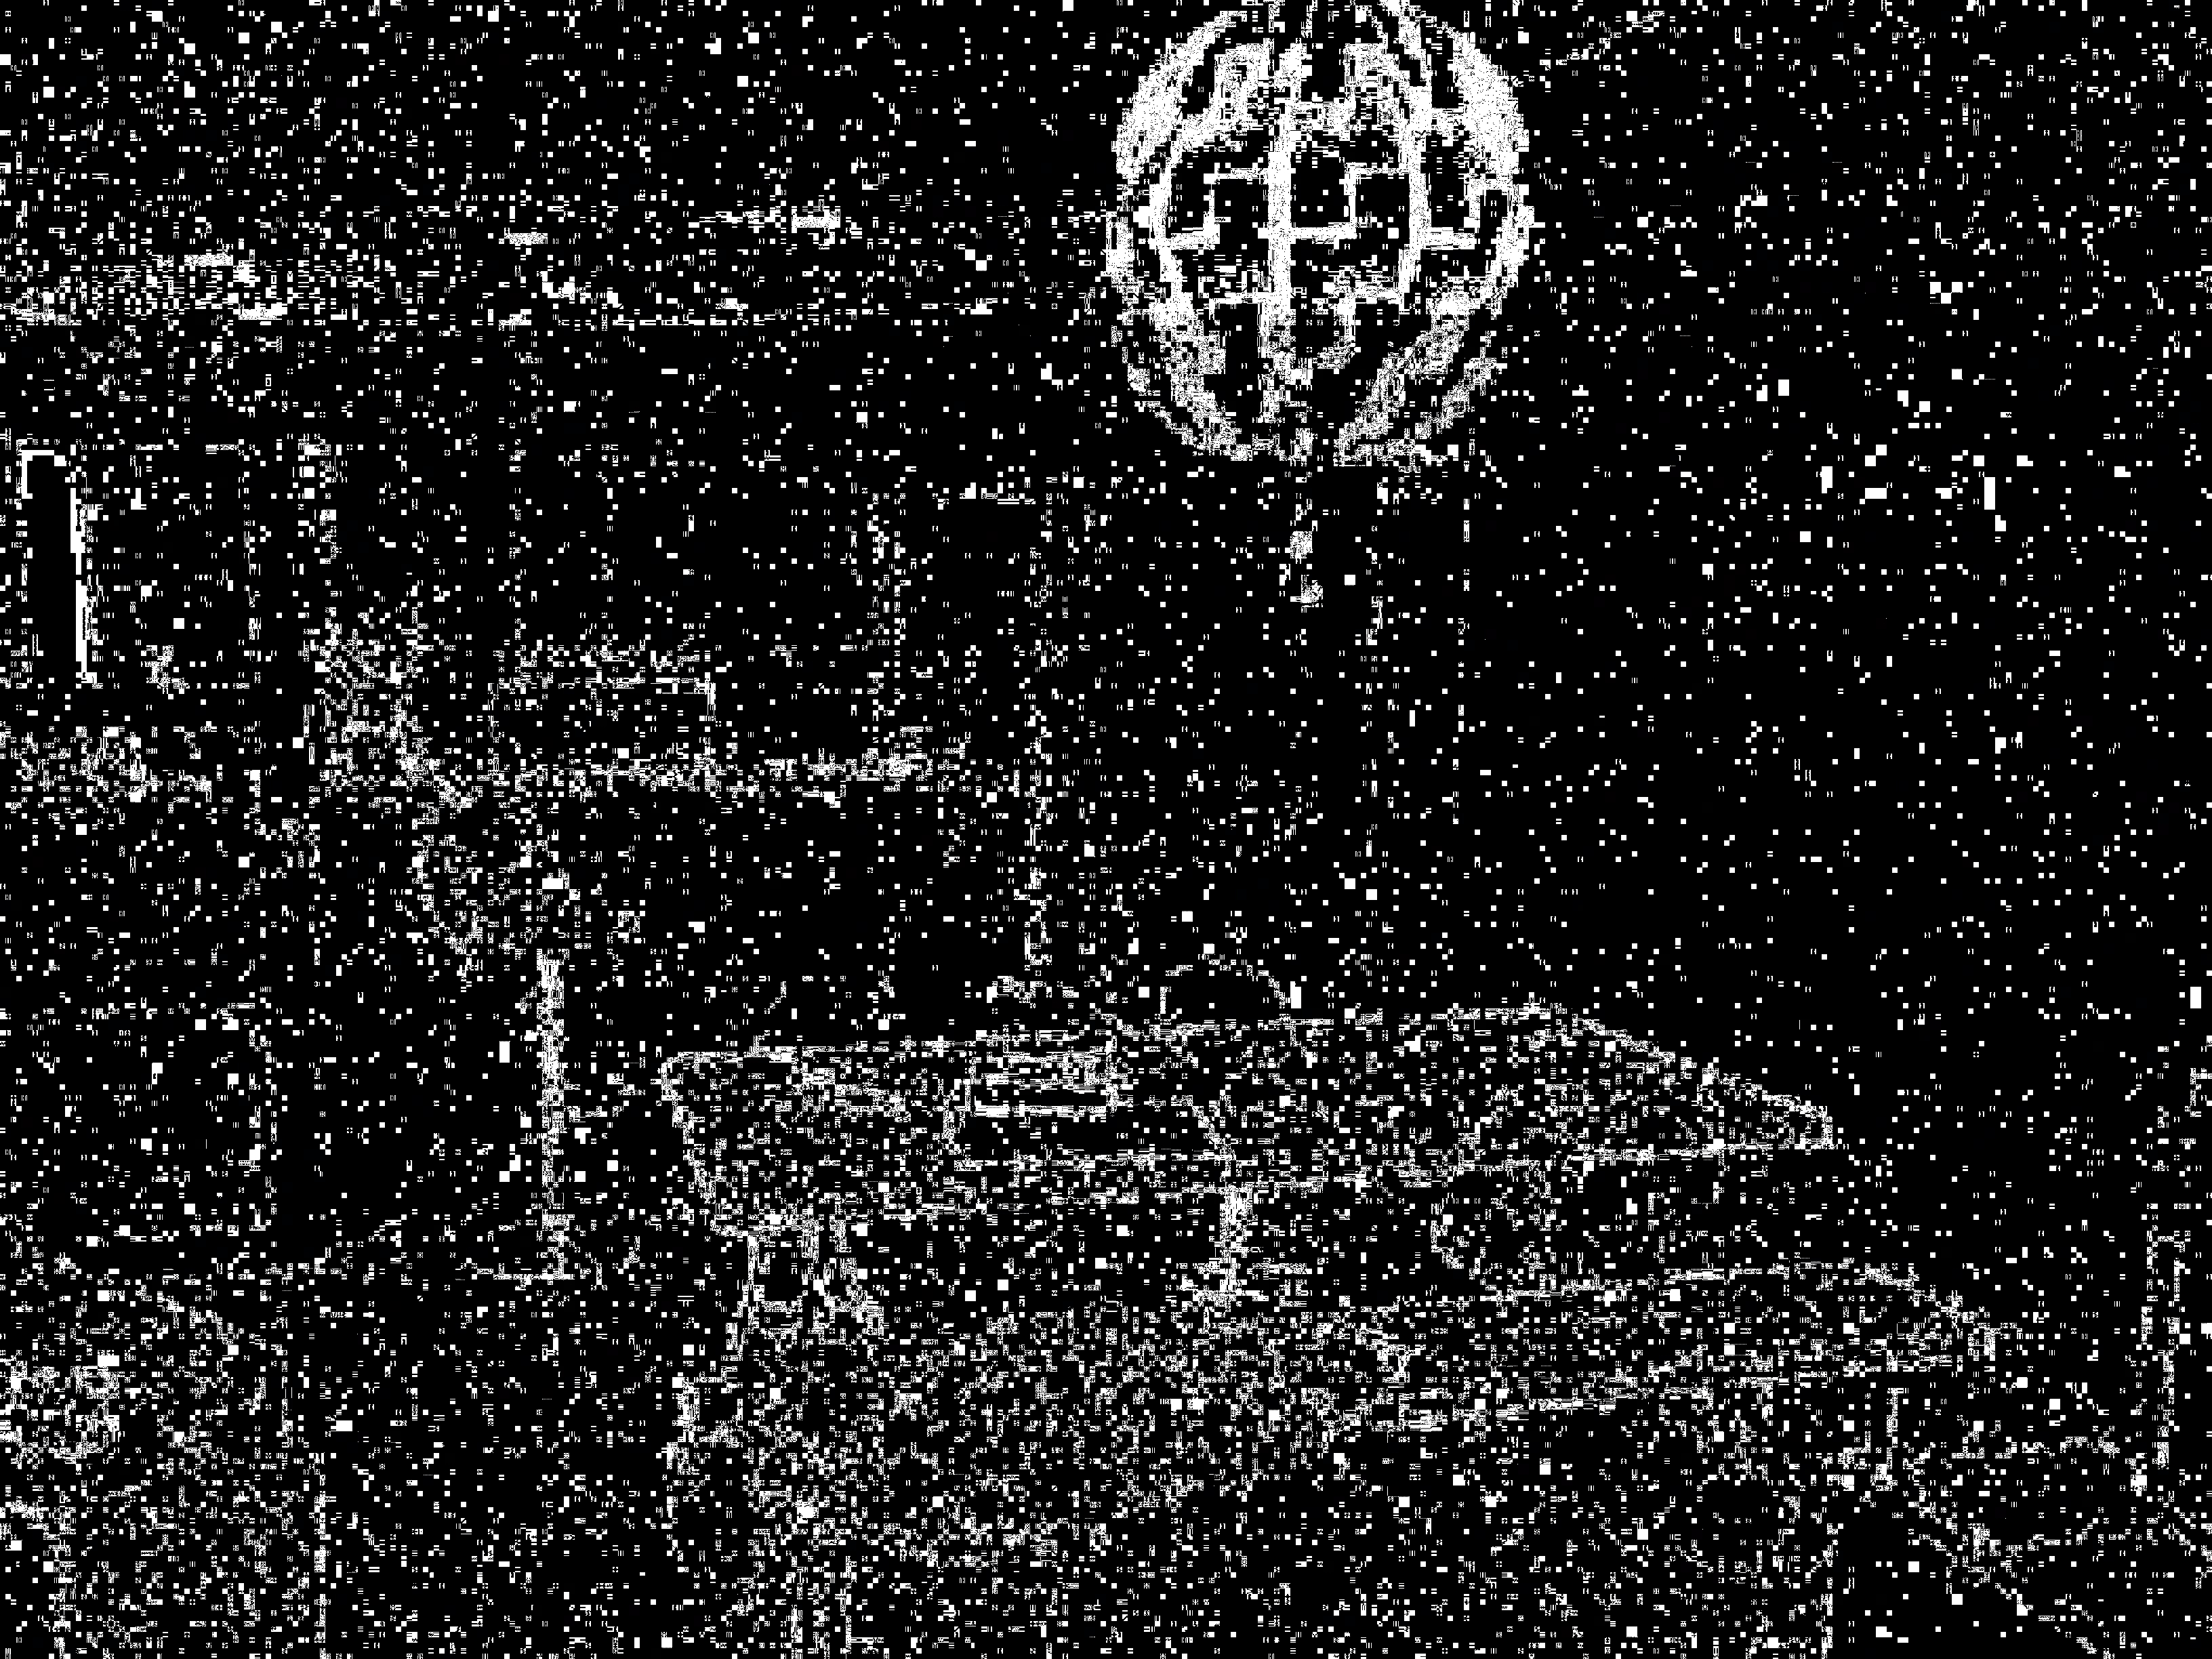
\includegraphics[width=.4\textwidth]{figures/introToStegovs1chardiff.jpg}}
\subfigure[RoomIntro]{\label{fig:a}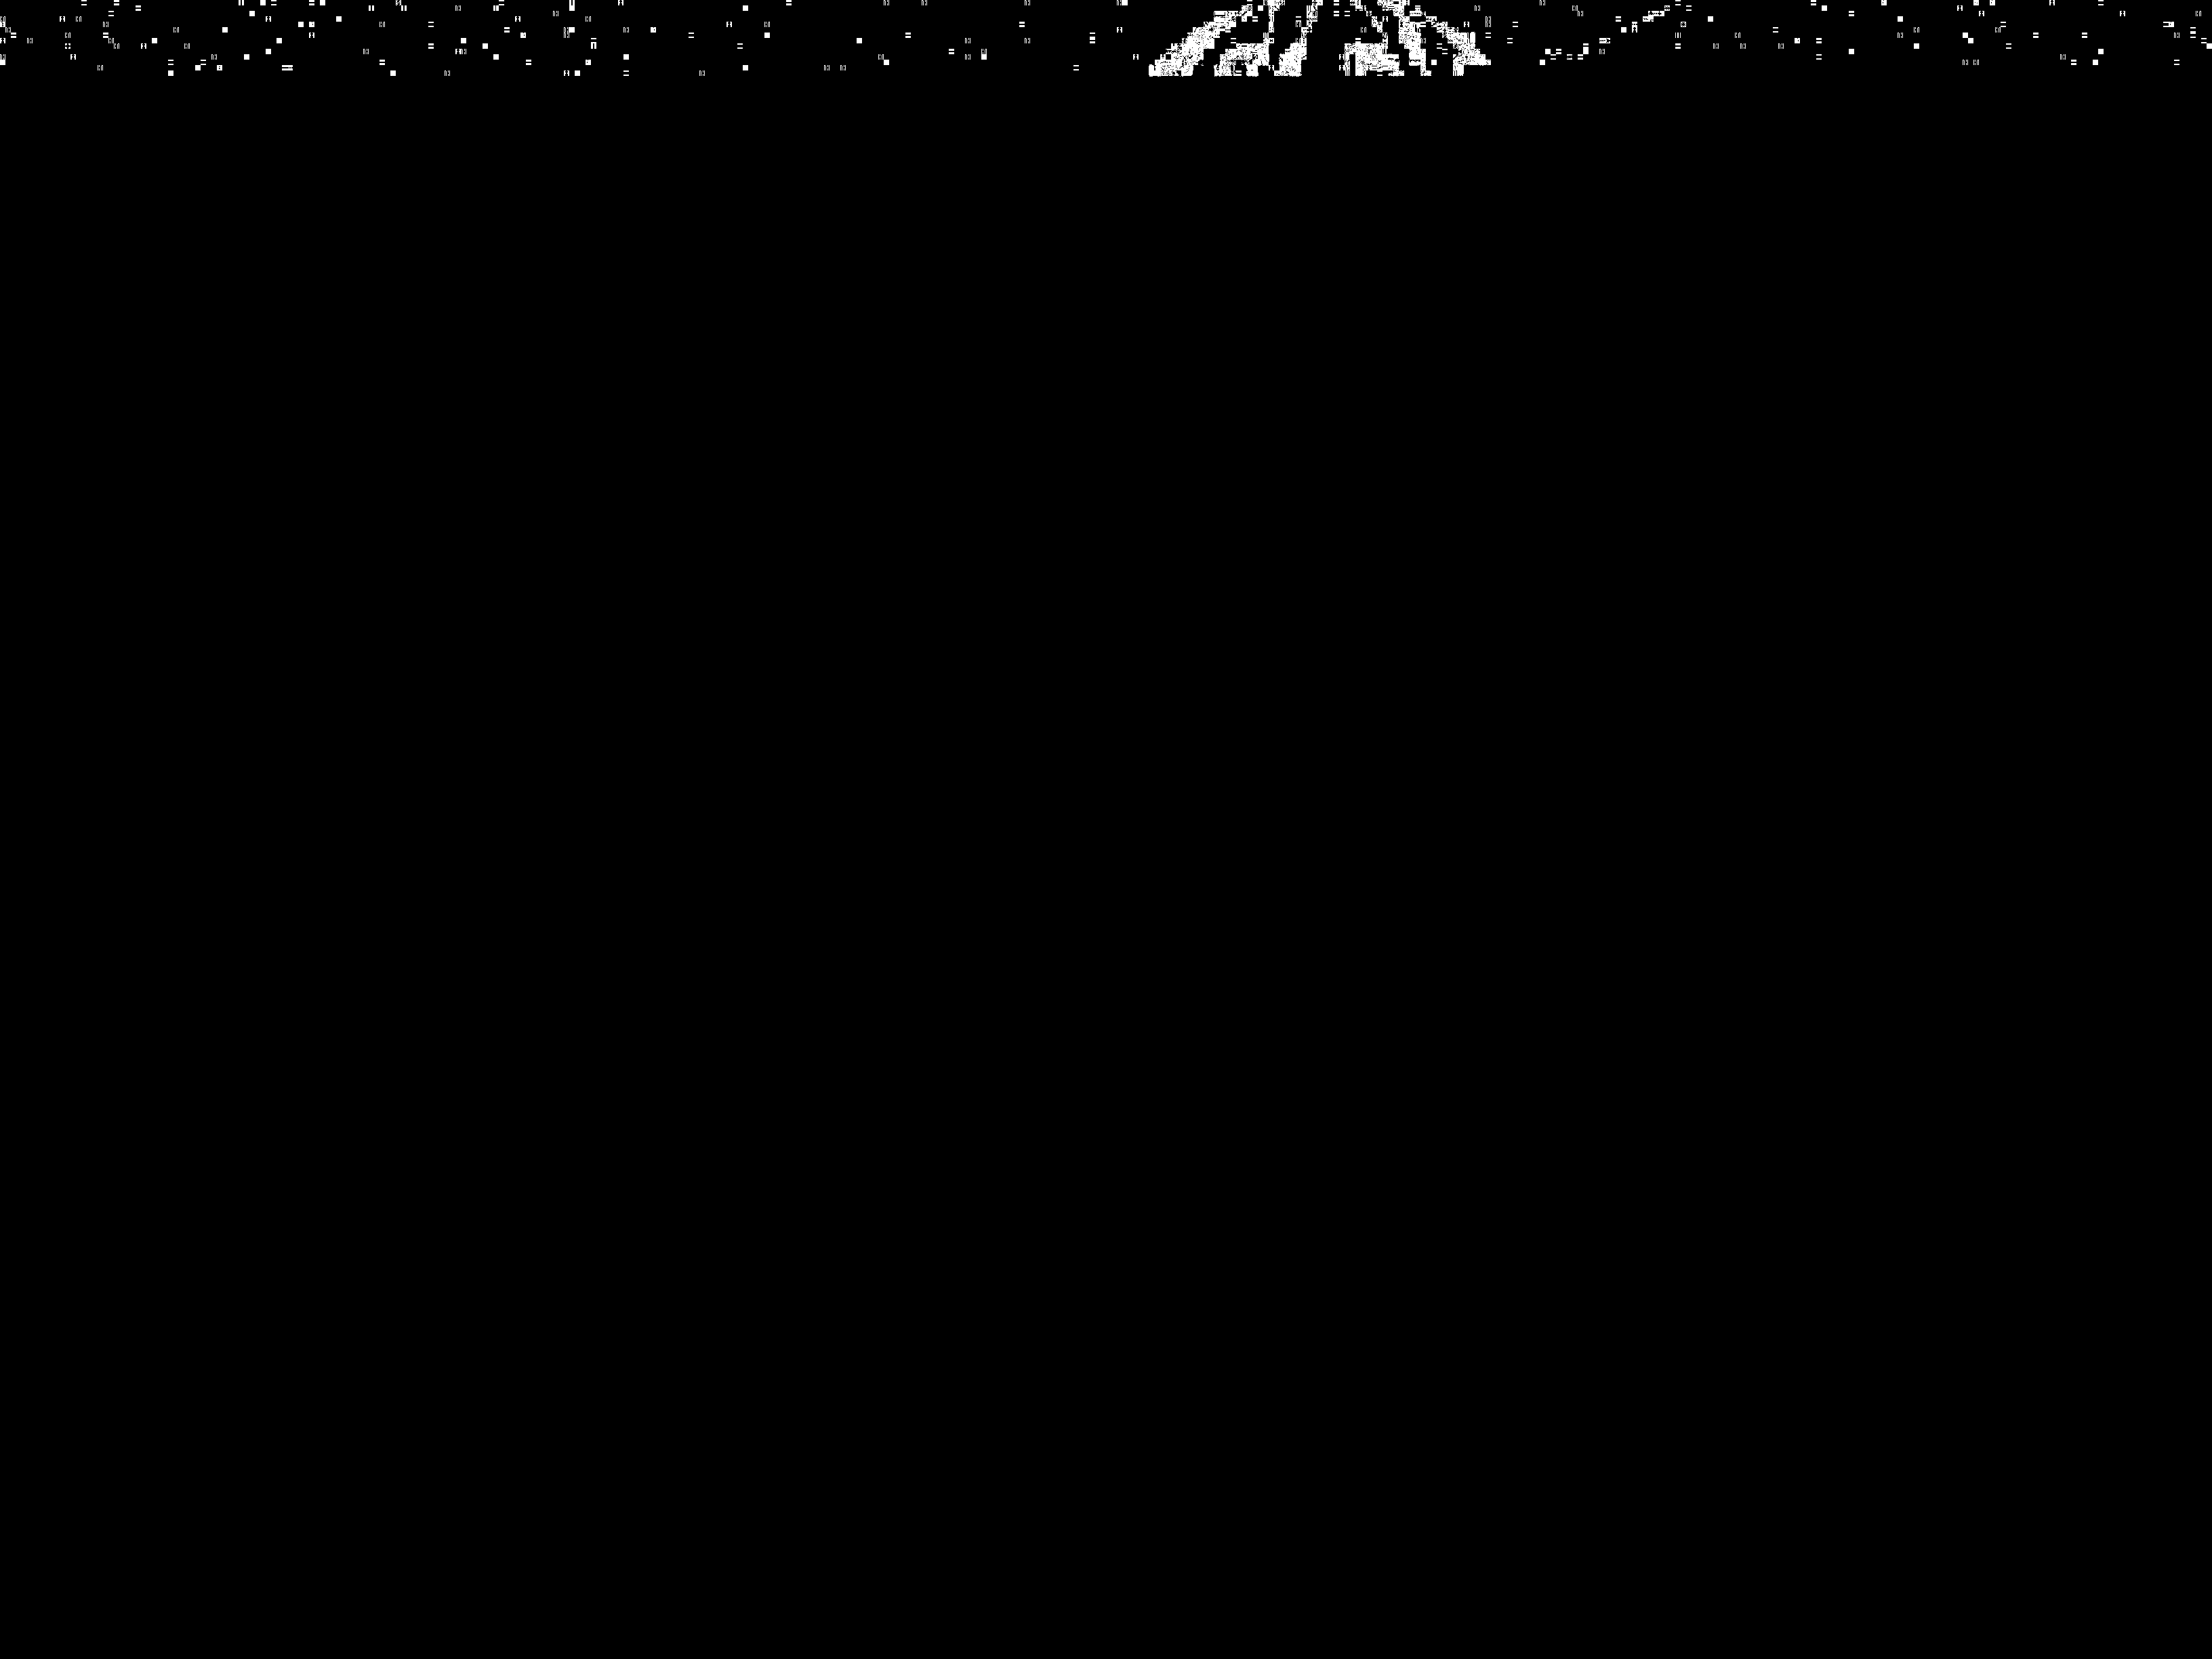
\includegraphics[width=.4\textwidth]{figures/loremIpsum1paragraphvs1chardiff.png}}
\caption{Sammenlligning af bileder}
\end{figure}
\end{frame}